
% Also note that the "draftcls" or "draftclsnofoot", not "draft", option
% should be used if it is desired that the figures are to be displayed in
% draft mode.
%
\documentclass[conference]{IEEEtran}
% Add the compsoc option for Computer Society conferences.
%

\usepackage{microtype}
\usepackage{comment}
\usepackage{booktabs}
\usepackage{fancyvrb}
\usepackage{comment}


% set typewrite font to be small
\fvset{fontsize=\small}

% *** CITATION PACKAGES ***
%
\usepackage{cite}
% cite.sty was written by Donald Arseneau
% V1.6 and later of IEEEtran pre-defines the format of the cite.sty package
% \cite{} output to follow that of IEEE. Loading the cite package will
% result in citation numbers being automatically sorted and properly
% "compressed/ranged". e.g., [1], [9], [2], [7], [5], [6] without using
% cite.sty will become [1], [2], [5]--[7], [9] using cite.sty. cite.sty's
% \cite will automatically add leading space, if needed. Use cite.sty's
% noadjust option (cite.sty V3.8 and later) if you want to turn this off.
% cite.sty is already installed on most LaTeX systems. Be sure and use
% version 4.0 (2003-05-27) and later if using hyperref.sty. cite.sty does
% not currently provide for hyperlinked citations.
% The latest version can be obtained at:
% http://www.ctan.org/tex-archive/macros/latex/contrib/cite/
% The documentation is contained in the cite.sty file itself.

% *** GRAPHICS RELATED PACKAGES ***
\usepackage[pdftex]{graphicx}
\graphicspath{{./data/}{./figs/}}
\DeclareGraphicsExtensions{.pdf,.jpg,.png}

% You can find documentation about the pdfTeX application at:
% http://www.tug.org/applications/pdftex





% *** MATH PACKAGES ***
%
\usepackage[cmex10]{amsmath}
% A popular package from the American Mathematical Society that provides
% many useful and powerful commands for dealing with mathematics. If using
% it, be sure to load this package with the cmex10 option to ensure that
% only type 1 fonts will utilized at all point sizes. Without this option,
% it is possible that some math symbols, particularly those within
% footnotes, will be rendered in bitmap form which will result in a
% document that can not be IEEE Xplore compliant!
%
% Also, note that the amsmath package sets \interdisplaylinepenalty to 10000
% thus preventing page breaks from occurring within multiline equations. Use:
%\interdisplaylinepenalty=2500
% after loading amsmath to restore such page breaks as IEEEtran.cls normally
% does. amsmath.sty is already installed on most LaTeX systems. The latest
% version and documentation can be obtained at:
% http://www.ctan.org/tex-archive/macros/latex/required/amslatex/math/





% *** SPECIALIZED LIST PACKAGES ***
%
%\usepackage{algorithmic}
% algorithmic.sty was written by Peter Williams and Rogerio Brito.
% This package provides an algorithmic environment fo describing algorithms.
% You can use the algorithmic environment in-text or within a figure
% environment to provide for a floating algorithm. Do NOT use the algorithm
% floating environment provided by algorithm.sty (by the same authors) or
% algorithm2e.sty (by Christophe Fiorio) as IEEE does not use dedicated
% algorithm float types and packages that provide these will not provide
% correct IEEE style captions. The latest version and documentation of
% algorithmic.sty can be obtained at:
% http://www.ctan.org/tex-archive/macros/latex/contrib/algorithms/
% There is also a support site at:
% http://algorithms.berlios.de/index.html
% Also of interest may be the (relatively newer and more customizable)
% algorithmicx.sty package by Szasz Janos:
% http://www.ctan.org/tex-archive/macros/latex/contrib/algorithmicx/




% *** ALIGNMENT PACKAGES ***
%
%\usepackage{array}
% Frank Mittelbach's and David Carlisle's array.sty patches and improves
% the standard LaTeX2e array and tabular environments to provide better
% appearance and additional user controls. As the default LaTeX2e table
% generation code is lacking to the point of almost being broken with
% respect to the quality of the end results, all users are strongly
% advised to use an enhanced (at the very least that provided by array.sty)
% set of table tools. array.sty is already installed on most systems. The
% latest version and documentation can be obtained at:
% http://www.ctan.org/tex-archive/macros/latex/required/tools/


\usepackage{mdwmath}
\usepackage{mdwtab}
% Also highly recommended is Mark Wooding's extremely powerful MDW tools,
% especially mdwmath.sty and mdwtab.sty which are used to format equations
% and tables, respectively. The MDWtools set is already installed on most
% LaTeX systems. The lastest version and documentation is available at:
% http://www.ctan.org/tex-archive/macros/latex/contrib/mdwtools/


% IEEEtran contains the IEEEeqnarray family of commands that can be used to
% generate multiline equations as well as matrices, tables, etc., of high
% quality.


%\usepackage{eqparbox}
% Also of notable interest is Scott Pakin's eqparbox package for creating
% (automatically sized) equal width boxes - aka "natural width parboxes".
% Available at:
% http://www.ctan.org/tex-archive/macros/latex/contrib/eqparbox/





% *** SUBFIGURE PACKAGES ***
%\usepackage[tight,footnotesize]{subfigure}
% subfigure.sty was written by Steven Douglas Cochran. This package makes it
% easy to put subfigures in your figures. e.g., "Figure 1a and 1b". For IEEE
% work, it is a good idea to load it with the tight package option to reduce
% the amount of white space around the subfigures. subfigure.sty is already
% installed on most LaTeX systems. The latest version and documentation can
% be obtained at:
% http://www.ctan.org/tex-archive/obsolete/macros/latex/contrib/subfigure/
% subfigure.sty has been superceeded by subfig.sty.



\usepackage{caption}
\usepackage[font=footnotesize]{subfig}
% subfig.sty, also written by Steven Douglas Cochran, is the modern
% replacement for subfigure.sty. However, subfig.sty requires and
% automatically loads Axel Sommerfeldt's caption.sty which will override
% IEEEtran.cls handling of captions and this will result in nonIEEE style
% figure/table captions. To prevent this problem, be sure and preload
% caption.sty with its "caption=false" package option. This is will preserve
% IEEEtran.cls handing of captions. Version 1.3 (2005/06/28) and later 
% (recommended due to many improvements over 1.2) of subfig.sty supports
% the caption=false option directly:
%\usepackage[caption=false,font=footnotesize]{subfig}
%
% The latest version and documentation can be obtained at:
% http://www.ctan.org/tex-archive/macros/latex/contrib/subfig/
% The latest version and documentation of caption.sty can be obtained at:
% http://www.ctan.org/tex-archive/macros/latex/contrib/caption/




% *** FLOAT PACKAGES ***
%
%\usepackage{fixltx2e}
% fixltx2e, the successor to the earlier fix2col.sty, was written by
% Frank Mittelbach and David Carlisle. This package corrects a few problems
% in the LaTeX2e kernel, the most notable of which is that in current
% LaTeX2e releases, the ordering of single and double column floats is not
% guaranteed to be preserved. Thus, an unpatched LaTeX2e can allow a
% single column figure to be placed prior to an earlier double column
% figure. The latest version and documentation can be found at:
% http://www.ctan.org/tex-archive/macros/latex/base/



%\usepackage{stfloats}
% stfloats.sty was written by Sigitas Tolusis. This package gives LaTeX2e
% the ability to do double column floats at the bottom of the page as well
% as the top. (e.g., "\begin{figure*}[!b]" is not normally possible in
% LaTeX2e). It also provides a command:
%\fnbelowfloat
% to enable the placement of footnotes below bottom floats (the standard
% LaTeX2e kernel puts them above bottom floats). This is an invasive package
% which rewrites many portions of the LaTeX2e float routines. It may not work
% with other packages that modify the LaTeX2e float routines. The latest
% version and documentation can be obtained at:
% http://www.ctan.org/tex-archive/macros/latex/contrib/sttools/
% Documentation is contained in the stfloats.sty comments as well as in the
% presfull.pdf file. Do not use the stfloats baselinefloat ability as IEEE
% does not allow \baselineskip to stretch. Authors submitting work to the
% IEEE should note that IEEE rarely uses double column equations and
% that authors should try to avoid such use. Do not be tempted to use the
% cuted.sty or midfloat.sty packages (also by Sigitas Tolusis) as IEEE does
% not format its papers in such ways.





% *** PDF, URL AND HYPERLINK PACKAGES ***
%
\usepackage{url}
% url.sty was written by Donald Arseneau. It provides better support for
% handling and breaking URLs. url.sty is already installed on most LaTeX
% systems. The latest version can be obtained at:
% http://www.ctan.org/tex-archive/macros/latex/contrib/misc/
% Read the url.sty source comments for usage information. Basically,
% \url{my_url_here}.

\usepackage[colorlinks = true,%
            linkcolor = blue,%
            urlcolor  = blue,%
            citecolor = blue,%
            anchorcolor = blue]{hyperref}



% *** Do not adjust lengths that control margins, column widths, etc. ***
% *** Do not use packages that alter fonts (such as pslatex).         ***
% There should be no need to do such things with IEEEtran.cls V1.6 and later.
% (Unless specifically asked to do so by the journal or conference you plan
% to submit to, of course. )


% correct bad hyphenation here
\hyphenation{op-tical net-works semi-conduc-tor}


\makeatletter
\g@addto@macro\@verbatim\small
\makeatother

\usepackage{authblk}
\renewcommand\Affilfont{\normalsize}
\renewcommand\Authfont{\normalsize}
\author[1]{Feiyi Wang}
\author[2]{Mark Nelson}
\author[1]{Sarp Oral}
\author[1]{Scott Atchley}
\author[2]{Sage Weil}
\author[1]{Brad Settlemyer}
\author[1]{Blake Caldwell}
\author[1]{Jason Hill}

\affil[1]{Oak Ridge National Laboratory, Oak Ridge, Tennessee 37831}
\affil[2]{Inktank Inc., Los Angeles, CA 90017}

\begin{document}
%
% paper title
% can use linebreaks \\ within to get better formatting as desired
\title{Performance and Scalability Evaluation of the \\Ceph Parallel File System}


% author names and affiliations
% use a multiple column layout for up to three different
% affiliations


\begin{comment}

\author{\IEEEauthorblockN{Michael Shell}
\IEEEauthorblockA{School of Electrical and\\Computer Engineering\\
Georgia Institute of Technology\\
Atlanta, Georgia 30332--0250\\
Email: http://www.michaelshell.org/contact.html}
\and
\IEEEauthorblockN{Homer Simpson}
\IEEEauthorblockA{Twentieth Century Fox\\
Springfield, USA\\
Email: homer@thesimpsons.com}
\and
\IEEEauthorblockN{James Kirk\\ and Montgomery Scott}
\IEEEauthorblockA{Starfleet Academy\\
San Francisco, California 96678-2391\\
Telephone: (800) 555--1212\\
Fax: (888) 555--1212}}

\end{comment}

% conference papers do not typically use \thanks and this command
% is locked out in conference mode. If really needed, such as for
% the acknowledgment of grants, issue a \IEEEoverridecommandlockouts
% after \documentclass

% for over three affiliations, or if they all won't fit within the width
% of the page, use this alternative format:
% 
%\author{\IEEEauthorblockN{Michael Shell\IEEEauthorrefmark{1},
%Homer Simpson\IEEEauthorrefmark{2},
%James Kirk\IEEEauthorrefmark{3}, 
%Montgomery Scott\IEEEauthorrefmark{3} and
%Eldon Tyrell\IEEEauthorrefmark{4}}
%\IEEEauthorblockA{\IEEEauthorrefmark{1}School of Electrical and Computer Engineering\\
%Georgia Institute of Technology,
%Atlanta, Georgia 30332--0250\\ Email: see http://www.michaelshell.org/contact.html}
%\IEEEauthorblockA{\IEEEauthorrefmark{2}Twentieth Century Fox, Springfield, USA\\
%Email: homer@thesimpsons.com}
%\IEEEauthorblockA{\IEEEauthorrefmark{3}Starfleet Academy, San Francisco, California 96678-2391\\
%Telephone: (800) 555--1212, Fax: (888) 555--1212}
%\IEEEauthorblockA{\IEEEauthorrefmark{4}Tyrell Inc., 123 Replicant Street, Los Angeles, California 90210--4321}}




% use for special paper notices
%\IEEEspecialpapernotice{(Invited Paper)}




% make the title area
\maketitle

\begin{abstract}

%Ceph is designed to be a reliable and scalable fault tolerant parallel file
%system with a number of intriguing features. 

Ceph is an emerging open-source parallel distributed file and storage
system. By design, Ceph is designed to leverage unreliable and commodity
storage and network hardware, and provides reliability and fault-tolerance
via controlled object placement and data replication.  
%Here we evaluate Ceph
%for scientific high-performance computing (HPC) environments.  
This paper
presents our file and block I/O performance and scalability evaluation of Ceph for
scientific high-performance computing (HPC) environments.
% methodology, experiments, results and observations from
%mostly parallel I/O performance and scalability perspectives.  
Our work makes
two unique contributions. First, our evaluation is performed under a realistic
setup for a large-scale capability HPC environment using a commercial
high-end storage system.
% (Data Direct Network's SFA10K).
%although typical in large-scale HPC environment, but atypical for average
%commercial off-the-shelf setup.  
Second, our path of investigation, tuning efforts, and findings made direct
contributions to Ceph's development and improved code quality, scalability, and
performance. These changes should benefit both Ceph and the HPC community
at large. 
%Throughout the evaluation, we observe that Ceph is an evolving
%technology under fast-paced development and shows great promises. 

\end{abstract}




% For peer review papers, you can put extra information on the cover
% page as needed:
% \ifCLASSOPTIONpeerreview
% \begin{center} \bfseries EDICS Category: 3-BBND \end{center}
% \fi
%
% For peerreview papers, this IEEEtran command inserts a page break and
% creates the second title. It will be ignored for other modes.
\IEEEpeerreviewmaketitle

\section{Introduction}

Oak Ridge Leadership Computing Facility (OLCF)\footnote{This research was
supported by, and used the resources of, the Oak Ridge Leadership Computing
Facility, located in the National Center for Computational Sciences at ORNL,
which is managed by UT Battelle, LLC for the U.S. DOE (under the contract No.
DE-AC05-00OR22725).} at Oak Ridge National Laboratory (ORNL) has a long history
of deploying and running very-large-scale high-performance computing (HPC)
systems\footnote{\url{http://www.top500.org/site/48553}}. The facility hosted
the Jaguar supercomputer up until recently, which was upgraded to the Titan
supercomputer. In order to satisfy the I/O demand of such supercomputers (as
well as, other OLCF computational, analysis, and visualization clusters), OLCF
also hosts large-scale file and storage systems. Lustre has been OLCF's choice
as the distributed parallel file system.  The latest incarnation of such
large-scale file systems hosted at OLCF is Spider II\cite{spider2}. Spider II
is the upgrade of its predecessor, Spider, which was deployed in 2008.
Spider II, deployed in 2013, is designed to operate at over 1 TB/s peak
aggregate I/O throughput and has a 40 PB of raw disk capacity. As the scratch
file system connected to a leadership computing platform at the scale of Titan,
Spider II emphasizes \textit{capability} over \textit{capacity}. However, we
also recognize that there are a wide variety of scientific data and workloads
with different performance and data access requirements (e.g., RESTful
interface, S3-like API, cloud solution integration) which might not be
efficiently serviced by Lustre. OLCF is constantly evaluating new and emerging
file and storage system technologies.  

Ceph\cite{Weil:2006:Ceph} is a distributed storage system designed for
scalability, reliability, and performance.  The system is based on a
distributed object storage service called RADOS (reliable autonomic distributed
object store) that manages the distribution, replication, and migration of
objects.  On top of that reliable storage abstraction Ceph builds a range of
services, including a block storage abstraction (RBD, or rados block device)
and a cache-coherent distributed file system (CephFS).

Data objects are distributed across storage daemons (ceph-osd) using
CRUSH\cite{crush}, a deterministic hashing function that allows administrators
to define flexible placement policies over a hierarchical cluster structure
(e.g., disks, hosts, racks, rows, datacenters).  Because the location of
objects can be calculated based on the object identifier and cluster layout
(similar to consistent hashing~\cite{..}), there is no need for a metadata
index or server for the RADOS object store. Further, because CRUSH provides an
authoritative view of data placement, storage daemons can coordinate directly
to handle data replications, recovery, or object migratation in the face of
failure or cluster topology changes.  A small cluster of monitors (ceph-mon
daemons) use Paxos to provide consensus on the current cluster layout, but do
not need to explicitly coordinate migration or recovery activities.

CephFS builds a distributed cache-coherent file system on top of the object
storage service provided by RADOS.  Files are striped over objects stored and
replicated by RADOS, while a separate cluster of metadata servers (ceph-mds
daemons) manage the file system namespace and coordinate client access to
files.  

Ceph metadata servers store all metadata in RADOS object, which provides a
shared, highly-available, and reliable storage backend.  Unlike many other
distributed file system architectures, Ceph also embeds inodes inside
directories in the common case, allowing entire directories to read from RADOS
into the metadata server cache or prefetched into the client cache using a
single request.

Client hosts that mount the file system communicate with one or more metadata
servers to traverse the namespace but perform file IO by reading and writing
directly to RADOS objects that contain the file data.  The metadata server
cluster monitors the temperature of cached metadata and periodically adjusts
the distribution of the namespace across the MDS cluster by migrating
responsibility for arbitrary subtrees of the hierarchy between a dynamic pool
of active ceph-mds daemons.  This dynamic subtree partitioning~\cite{..}
strategy is both adaptive and highly scalable, allowing additional metadata
server daemons to be added or removed at any time, making it ideally suited
both for large-scale workloads with bursty workloads or general purpose
clusters whose workloads grow or contract over time.

\begin{comment}
In comparison to other parallel file
systems, Ceph has a number of distinctive features:

\begin{itemize}
 
\item Ceph has an intelligent and powerful data placement mechanism, known as
  CRUSH. The CRUSH algorithm allows a client to pre-calculate object
  placement and layout while taking into consideration of failure domains and
  hierarchical storage tiers.
  
  \item From the start, Ceph's design anticipated managing meta data and the
  name space with a cluster of meta data servers. It utilized a dynamic subtree
  partitioning strategy to continuously adapt meta data distribution to current
  demands.

  \item Ceph's design assumes that the system is composed of unreliable
  components; fault-detection and fault-tolerance (e.g., replication) are the
  norm rather than the exception. This is in line with the expectations and
  future directions of Exascale computing.

  \item Ceph is built on top of a unified object management layer, RADOS. Both
  meta data and the file data can take advantage of this uniformity. On top of
  RADOS, Ceph build and project a host of other features such as RESTful
  interface, S3 and Swift-compliant API, cloud integration.

  \item Most of the Ceph processes reside in user-space. Generally speaking,
this makes the system easier to debug and maintain. The client-side support has
long been integrated into Linux mainline kernel, which eases the deployment and
out-of-box experience.

\end{itemize}
\end{comment}

As interesting and feature-rich as Ceph may be,  scalability and performance
are our top priorities due to the unique requirements our environment.  As part
of this study, we set up a dedicated testbed within OLCF to  evaluate Ceph.
Our goal was to investigate the feasibility of using the Ceph for future
large-scale scientific HPC storage deployments. This paper presents our
experience, results, and observations.  While evaluating our results, please
keep in mind that Ceph is still a relatively \textit{young} parallel file
system and its code base is changing rapidly. In between releases, we often
experienced different stability and performance outcomes.  We will try to make
clear in the writing when such changes occurred.

This paper is organized as follows. Section~\ref{sec:testbed} gives an
overview on our general test and evaluation methodology as well as testbed
environment; Following it, Section~\ref{sec:baseline} establishes the baseline
performance and expectations for all critical components on the data path;
Section~\ref{sec:ceph-initial} discusses our early runs, results, and issues
bottom up: from middle tier RADOS object layer to the file system-level and
then meta data performance. In Section~\ref{sec:ceph-tuning} we highlight the
investigative and tuning effort, we compare results before and after, and how
the process eventually bring the system performance to a respectable state.
Finally, Section~\ref{sec:conclusion} summarizes our findings, observations,
and future works.

\section{Testbed Environment Description}
\label{sec:testbed}

We used Data Direct Networks' (DDN) SFA10K as the storage backend for this
evaluation. SFA10K organizes disks into various RAID levels by two
active-active RAID controllers. The exported RAID groups (LUNs) by these
controllers are driven by four server hosts (oss-[1-4]).  Each server host has two InfiniBand
(IB) QDR connections to the storage backend.  We used a single dual-port
Mellanox ConnectX IB QDR card per host.  By our calculation, this setup is
adequate to drive the SFA10K at its maximum theoretical throughput (roughly 12
GB/s). Server hosts and SFA10K connection diagram is illustrated in
Figure~\ref{fig:ddn-sfa10k}.

\begin{figure}[htb]
\centering
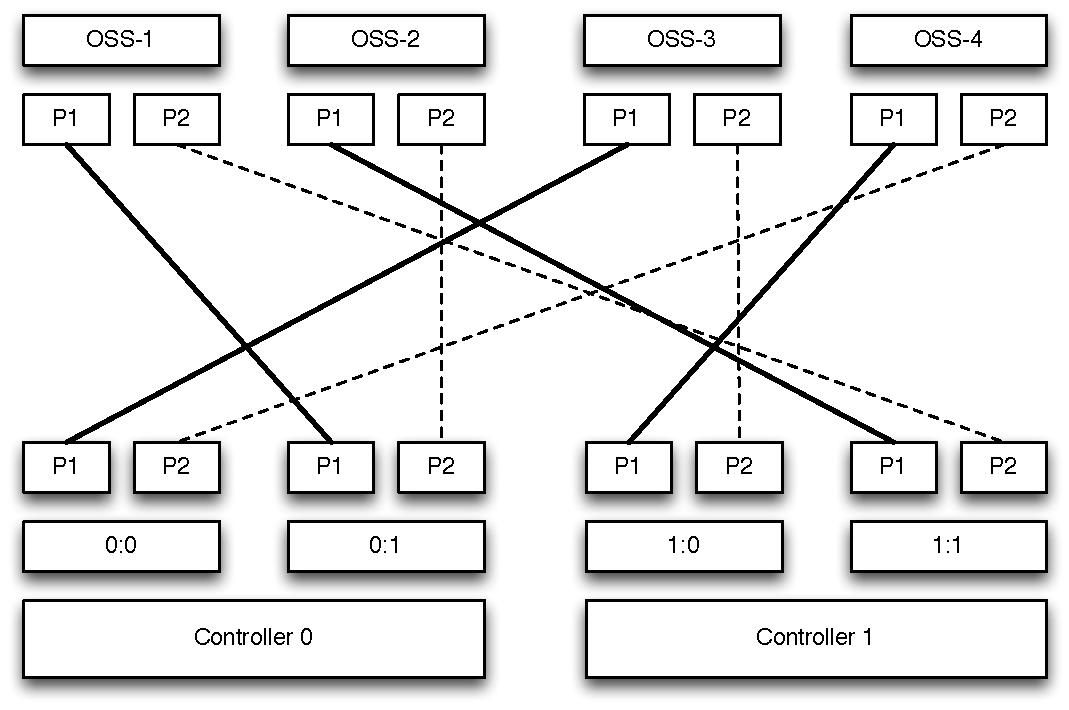
\includegraphics[width=3in]{figs/sfa10k}
\caption{DDN SFA10K hardware and host connection diagram}
\label{fig:ddn-sfa10k}
\end{figure}


Our SFA10K system consists of 200 SAS drives and 280 SATA drives, hosted in a
10-tray configuration. Each DDN SA4601 disk tray can host up to 60 disks and
has two SAS links per controller (four in total). The SATA and SAS disks in our
testbed are distributed evenly over ten SA4601 disk trays (20 SAS and 28 SATA
disks per tray). Each SFA10K RAID controller has two RAID processors and each
RAID processor hosts a dual-port IB QDR card. The disks are organized into RAID
groups by the RAID processors (software RAID) and then exported to connected
server hosts over the IB connections. Since each DDN SFA10K controller is a
stand-alone computer system running Linux, CPU and memory affinity while
organizing disks into RAID groups and exporting them is crucial for obtaining
top performance out of an SFA10K system.  

Our Ceph testbed employs a collection of nodes, including the server hosts
(oss-[1-4]). These nodes and their roles are summarized in
Table~\ref{tbl:ceph-test-nodes}. In the following discussion, we use
``servers'', ``osd servers'', ``server hosts'' interchangeably. We will
emphasize with ``client'' prefix when we want to distinguish it from above.

\begin{table}[!t]
\centering
\caption{Support nodes involved in Ceph testbed}
\label{tbl:ceph-test-nodes}
    \begin{tabular}{ll}
    \hline
    Node & Role \\
    \hline
    tick-mds1 & Ceph monitor node \\
    spoon46 & Ceph MDS node \\
    tick-oss[1-4] & Ceph OSD servers \\
    spoon28-31, spoon37-41 & Ceph client nodes \\
    \hline
    \end{tabular}
\end{table}

All hosts  (client and servers) were configured with Redhat 6.3 and kernel
version 3.5.1 initially, and later upgraded to 3.9 (rhl-ceph image), Glibc
2.12 with syncfs support, locally patched.  We used the Ceph 0.48 and 0.55
release in the initial tests, upgraded to 0.64 and then to 0.67RC for a final
round of tests.

%For a complete a list of hosts that are running ceph images, one can execute:

%\begin{Verbatim}
%$ grep "rhel6-ceph" /etc/gedi/MAC.info
%\end{Verbatim}


Our testing methodology is bottom to top. We start our evaluation from the
lowest level (i.e. block-level)  to establish a baseline performance and work
our way up to the top (i.e. file system-level). We establish an expected
theoretical performance of a given hardware or software layer and then compare
that with the observed results of our experiments. Each added new layer to the
stack introduces new bottlenecks and re-defines the expected theoretical
performance of the overall system. We will explain each component or layer and
its expected performance before we present our observed results.

Our tools for benchmarking and evaluating different layers also change as we go
up in the stack.  For example, a tool perfect for assessing block-level
performance over a single server host might be completely inadequate for
observing parallel file system performance over multiple clients. As we present
our evaluations, we will also introduce and explain our benchmark tools, in
this paper.

\section{Establishing A Baseline Performance}
\label{sec:baseline}

\subsection{Block I/O over Native IB} 

The lowest layer in the system are the exposed LUNs to the server hosts from
the RAID controllers.  These LUNs are mostly configured as a RAID6 8+2 array (8
data disks and 2 \textit{P} and \textit{Q} disks). In our earlier tests we
observed that a 7.2K RPM SAS disk can perform at ~140 MB/s for 128 kB
sequential I/O requests and a 7.2K RPM SATA disk can do ~36 MB/s. For these
tests, all disk caches were turned off. Therefore, in 8 data disk RAID group
with 1 MB sequential I/O requests (each disks sees 128 kB chunks of the
request) the expected aggregate performance would be ~1.12 GB/s for a SAS RAID
group and ~288 MB/s for a SATA RAID group, if there are no caches along the I/O
path.  With the caches turned on, especially the write-back cache on the DDN
RAID controller, we observe a significant performance improvement. In our
day-to-day HPC operations we run our storage systems with write-back cache
turned on on RAID controllers, if and only if, there is a method of
cache-mirroring between the two active-active RAID controllers to recover from
a single controller failure scenario. With the write-back cache on we observe
~1.4 GB/s per RAID 6 8+2 SAS group and ~955 MB/s per RAID 6 8+2 SATA group, for
1 MB sequential I/O. These two performance numbers will be used as a baseline
in our study and they are presented in Table~\ref{tbl:block-io-baseline}.  For
these tests, the 8+2 RAID 6 groups are exported to the server hosts using SCSI
RDMA Protocol (SRP) over IB protocol (which is the default for our normal HPC
configurations). For a SATA disk group this translates into roughly 120
MB/s/disk and for a SAS disk group it is 175 MB/s. As can be seen, SATA RAID
groups benefit from caching more than SAS groups. 

For above tests the RAID groups are exported over physical 4x IB QDR links.
These links can provide up to 40 Gbits/s signalling rate and 32 Gbits/s actual
data rate (reduction is due to 8/10 encoding scheme). Therefore, each IB QDR
link can perform at 3.2 GB/s, while in practice we see around 3 GB/s as the
best case. 

As mentioned earlier, we had 280 SATA disks and 200 SAS disks. Organizing these
into RAID 6 8+2 groups will yield 28 SATA and 20 SAS RAID 6 8+2 groups. We had
4 server hosts in our testbed and evenly distributing these on to 4 server
hosts translates into 8 SATA LUNs and 4 SAS LUNs per server host (when a RAID
group is exported to a server host, it is labeled as a LUN from the server host
point of view).

Next, we established the baseline performance for a single server host. We
exercised all seven SATA LUNs concurrently form a single server host at the
block-level. This resulted in an aggregate performance of roughly 2.6 GB/s.
Repeating the same test using only four SAS LUNs yielded around 2.8 GB/s
aggregate performance for 1 MB sequential I/O. These two numbers will be used
as single server host aggregate baseline performance for this study. These are
also presented in presented in Table~\ref{tbl:block-io-baseline}. 

It is worth mentioning that we used our in-house developed synthetic benchmark,
\textit{fair-lio} for all our block-level testing.  fair-lio has better
sequential I/O characteristics compared to commonly used XDD benchmark and it
is asynchronous and based on the Linux libaio library.


\begin{table}[htb]
\centering
\caption{Block I/O performances on single LUN and single host}
\label{tbl:block-io-baseline}

\begin{tabular}{| l | l |}
    \hline
    SAS single LUN sequential read & ~1.4 GB/s \\
    SATA single LUN sequential read & ~955 MB/s \\
    Single host with four SAS LUNs & ~ 2.8 GB/s \\
    Single host with seven SATA LUNs & ~ 2.6 GB/s \\
    \hline
\end{tabular}
\end{table}

When exercising all 28 SATA LUNs from all four server hosts in parallel, we
observed an 11 GB/s aggregate performance. Same level of performance was
observed using all 20 SAS LUNs from four server hosts in parallel. Comparing
these to the advertised peak performance of 12 GB/s of the DDN SFA10K, we
concluded that our test setup is well configured to drive the backend disk
system at full performance and we are limited by the RAID controller
performance. Going forward in this study, 11 GB/s will be used the peak
baseline for the entire test configuration.


\subsection{Establishing an IP over IB Baseline Performance}

Ceph uses the BSD Sockets interface in \texttt{SOCK\_STREAM} mode (i.e., TCP).
Because our entire testbed is built on IB QDR fabric (including client to
server host connections over a 108-port Mellanox IB QDR switch), we used IP
over IB (IPoIB) for networking\footnote{As of writing of this report, Inktank
is investigating using rsockets to improve performance with IB fabric}. Through
simple \verb!netperf! tests, we observed that a pair of hosts connected by IB
QDR using IPoIB can transfer data at 2.7 GB/s (the hosts are tuned per
recommendations from Mellanox). With all four server hosts (OSD servers), we
expect the aggregate throughput to be in the neighborhood of 11 GB/s.

Unfortunately there was not enough time to do more detailed analysis of the
network performance. However, as we observed later, RADOS is performing no
more than 8 GB/s driven by four server hosts. This confirms that we have
provisioned enough network bandwidth. In other words, IP over IB is not a
bottleneck in this case.


\section{Ceph RADOS Scaling: Initial Results}

RADOS is a reliable distributed object store, the foundational component for
CephFS file system. There are two types of scaling tests we are interested at
the RADOS layer:

\begin{itemize}
  \item scaling on the number of OSD servers
  \item scaling on the number of OSDs per OSD server
\end{itemize}

Our system setup poses some limitations on the scalability tests we wanted to
perform. In particular, we currently had four OSD servers, eight clients, and
eleven OSD servers per client. The scaling tests, therefore, will be within
these constraints.

We used the open-source RADOS Bench tool, developed by Inktank, to perform our
initial performance analysis of the underlying RADOS layer.  RADOS Bench simply
writes out objects to the underlying object storage as fast as possible, and
then later reads those objects in the same order as they were written.

We observed that using two or more client processes and many concurrent
operations are important when performing these tests.  We tested eight client processes 
with 32 concurrent 4 MB objects in flight each. We created a pool for
each RADOS Bench process to ensure that object reads come from independent pools
(RADOS Bench is not smart enough to ensure that objects are not read by multiple
processes and thus possibly cached).  A sync and flush is performed on every
node before every test to ensure no data or metadata is in cache.  All tests
were run with replication set to one.  The backend file systems were XFS,
BTRFS and EXT4 file systems were not tested at this time.


\subsection{Scaling on number of OSDs per server}

In the following test, a single Ceph host drives $n$ OSDs, where $n$ increases
from one to eleven. The result is illustrated in Figure~\ref{fig:osd-scale}.
We ran the test against a single client with four concurrent processes. In this
test case, we observe that the OSD server exhibits near linear scalability up to
nine OSDs, and is still trending upwards at eleven OSDs. This suggests that we
have not reached the saturation point yet. Additional testing would require
provisioning more OSDs on the SFA10K backend.


\begin{figure}[!t]
\centering
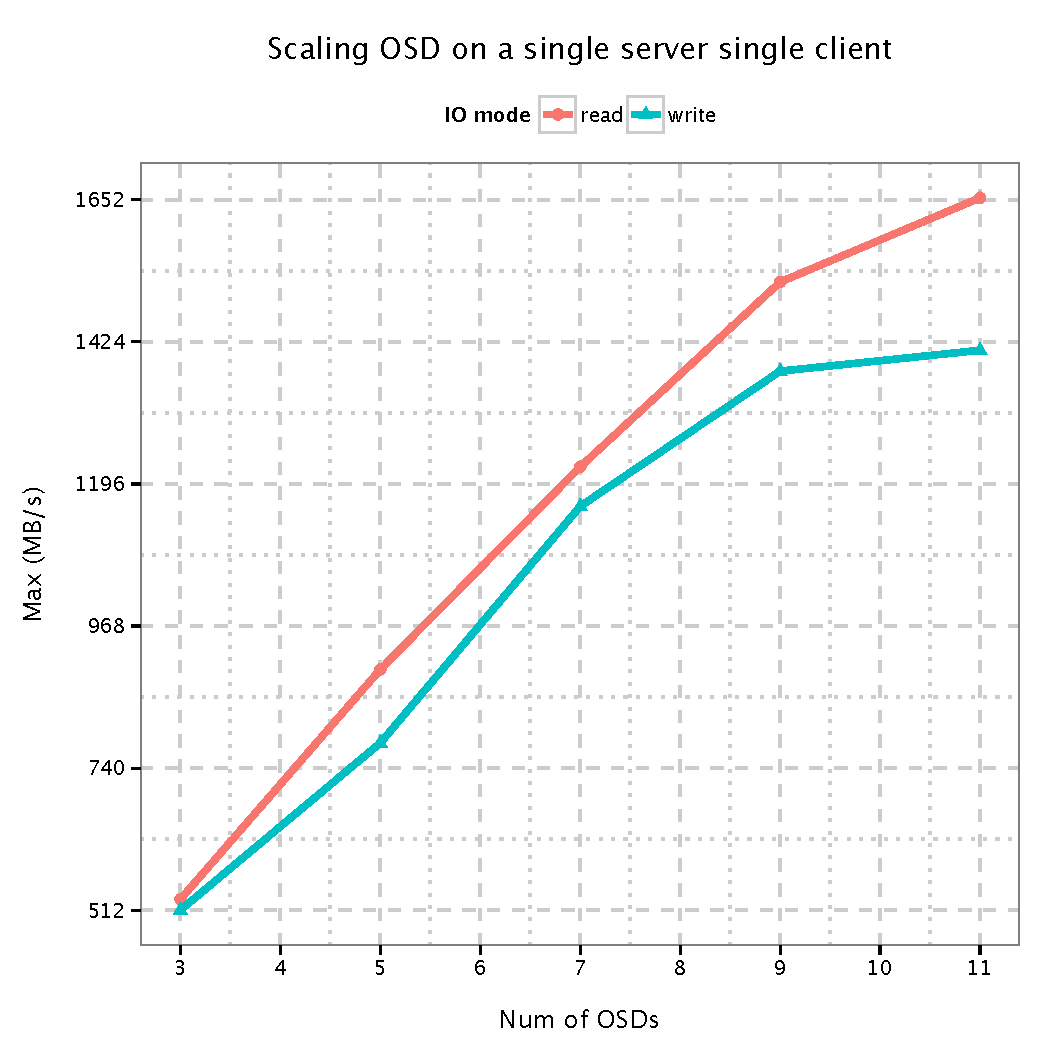
\includegraphics[width=3in]{data/rados_osd}
\caption{RADOS scaling on number of OSDs}
\label{fig:osd-scale}
\end{figure}

\begin{figure}[!t]
\centering
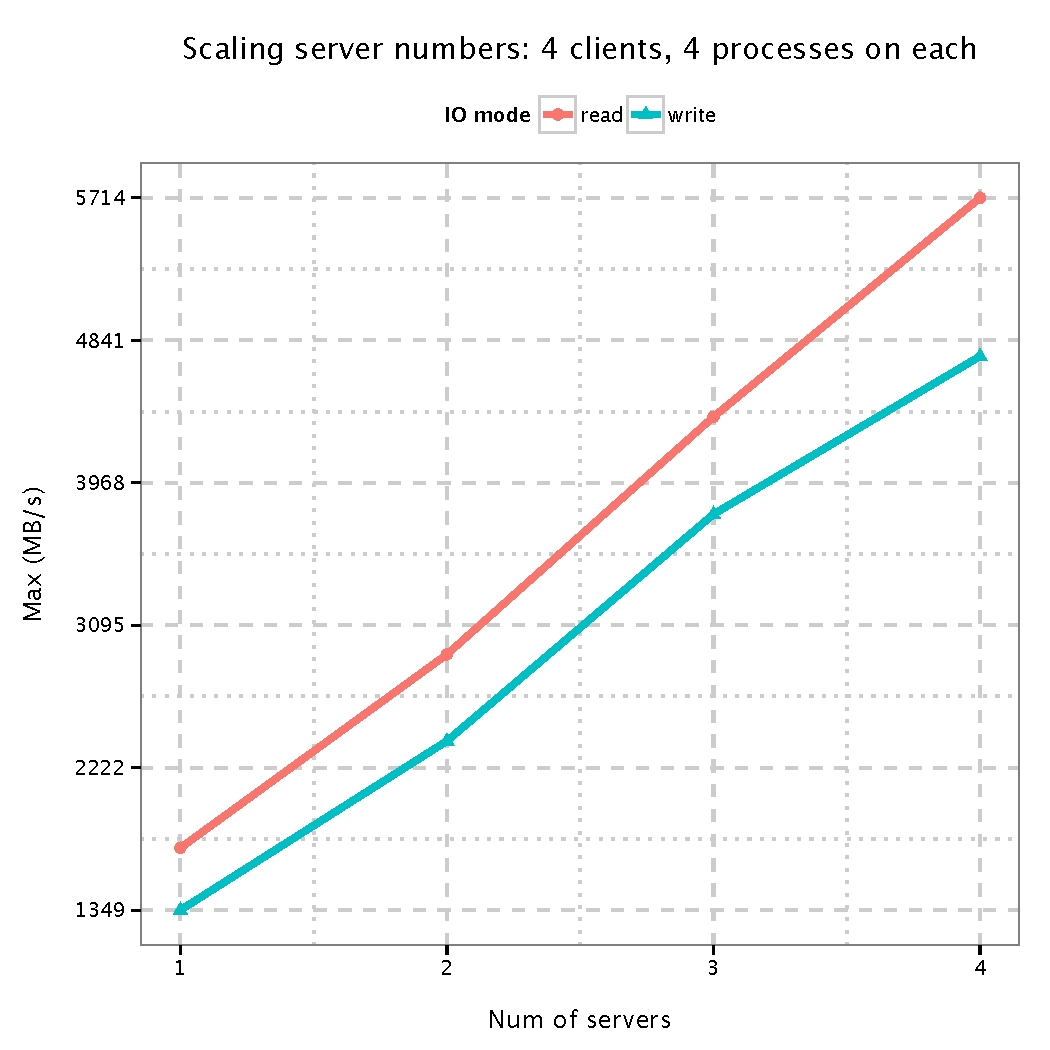
\includegraphics[width=3in]{data/rados_server}
\caption{RADOS scaling on number of servers}
\label{fig:oss-scale}
\end{figure}

\subsection{Scaling on number of OSD servers}

In this test, we exercise OSD servers from one to four, driven by four hosts
each with four RADOS Bench process. Each additional OSD server
adds eleven more OSDs into play. We observe that Ceph exhibits linear scaling with
regard to number of servers as well, at least in the given set of servers.
However, the peak performance we are seeing is about the half of what are
expecting from the SFA10K (compare to the baseline block I/O perforamnce number
presented in Section~\ref{sec:block-io}).

For writes, the lost performance is attributed to the way Ceph performs
journaling:
Ceph does not support meta-data only journaling, therefore every write is the
equivalent of a double-write: once to the data device, once to the journaling
device. This effectively cuts the observed system bandwidth in half. That said,
it does not explain the read performance -- it is a little better than write,
but still far from the theoretical maximum.

\section{Ceph File System Performance: Initial Test}
\label{sec:ior-initial}
We used the synthetic IOR benchmark suite for file system level performance and
scalability test.
The particular parameter setup is show in Table \ref{tbl:ior}. Each client node
has 6 GB of physical memory, the block size is set so as to mitigate cache
effects. In addition, the test harness program issues the following commands
at the beginning of each test:




\begin{table}[tb]
\caption{IOR parameter setup}
\label{tbl:ior}
\centering
\begin{tabular}{p{0.8in} | p{2in}}
    \hline
    IOR parameter & Note \\ \hline
    \verb!-F! & file per process \\ \hline
    \verb!-a POSIX! & use POSIX API \\ \hline
    \verb!-w -r -C! & do both write and read test, \verb!-C! is to change task
        ordering for read back so it will not read from the write cache. \\
        \hline
    \verb!-i 3 -d 5! & 3 iterations and delay 5 seconds betewen iterations \\ \hline  
    \verb!-e! & perform \verb!fsync()! upon POSIX write close \\ \hline
    \verb!-b 8g or 16g! & the block size \\ \hline
    \verb!-t 4k to 4m! & the transfer size \\ \hline
    \verb!-o file! & mandatory test file  \\    
    \hline
\end{tabular}
\end{table}


\begin{Verbatim}
# sync
# echo 3 | tee /proc/sys/vm/drop_caches
\end{Verbatim}


Here, 0 is the default value of \verb!drop_caches!; 1 is to free pagecaches, 2
is to free dentries and inodes, 3 is to free pagecache, dentries, and inodes.


Our first round of tests was less than ideal as we encountered various issues. For
the sake of completeness, we first summarize the results, then discuss
further tuning efforts and improvements.

The full permutation of IOR parameters were not explored due to I/O errors we encountered.
We were, however, able to record results in two extreme cases as far as
transfer size is concerned: 4 KB and 4 MB, using a fixed number of OSD servers
(4) and fixed block size (8 GB), the results are illustrated in Figure
\ref{fig:ior4k} and \ref{fig:ior4m}, we make the following observations:


\begin{figure*}[!t]

\centerline{\subfloat[4 KB transfer size]
{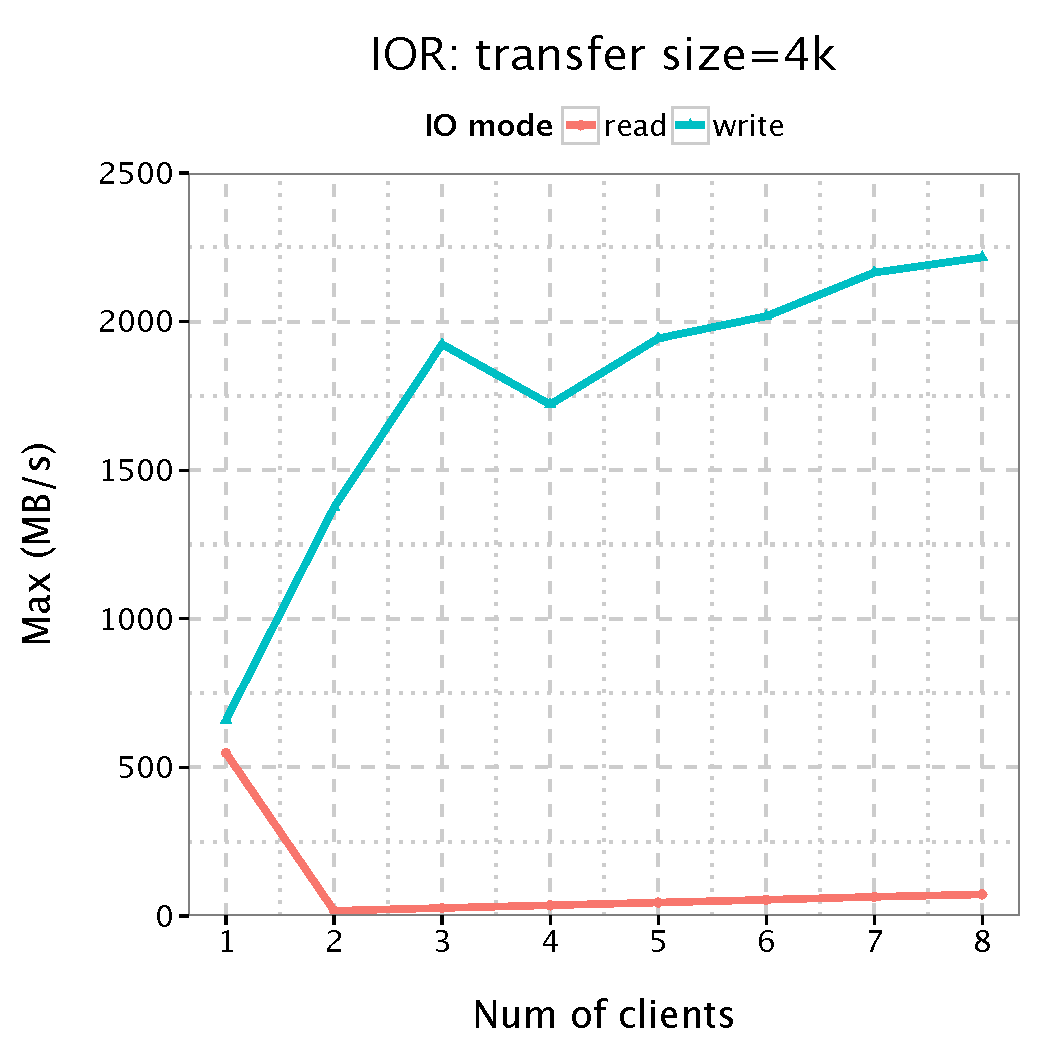
\includegraphics[width=3in]{data/ior_4k}
\label{fig:ior4k}}
\hfil
\subfloat[4 MB transfer size]
{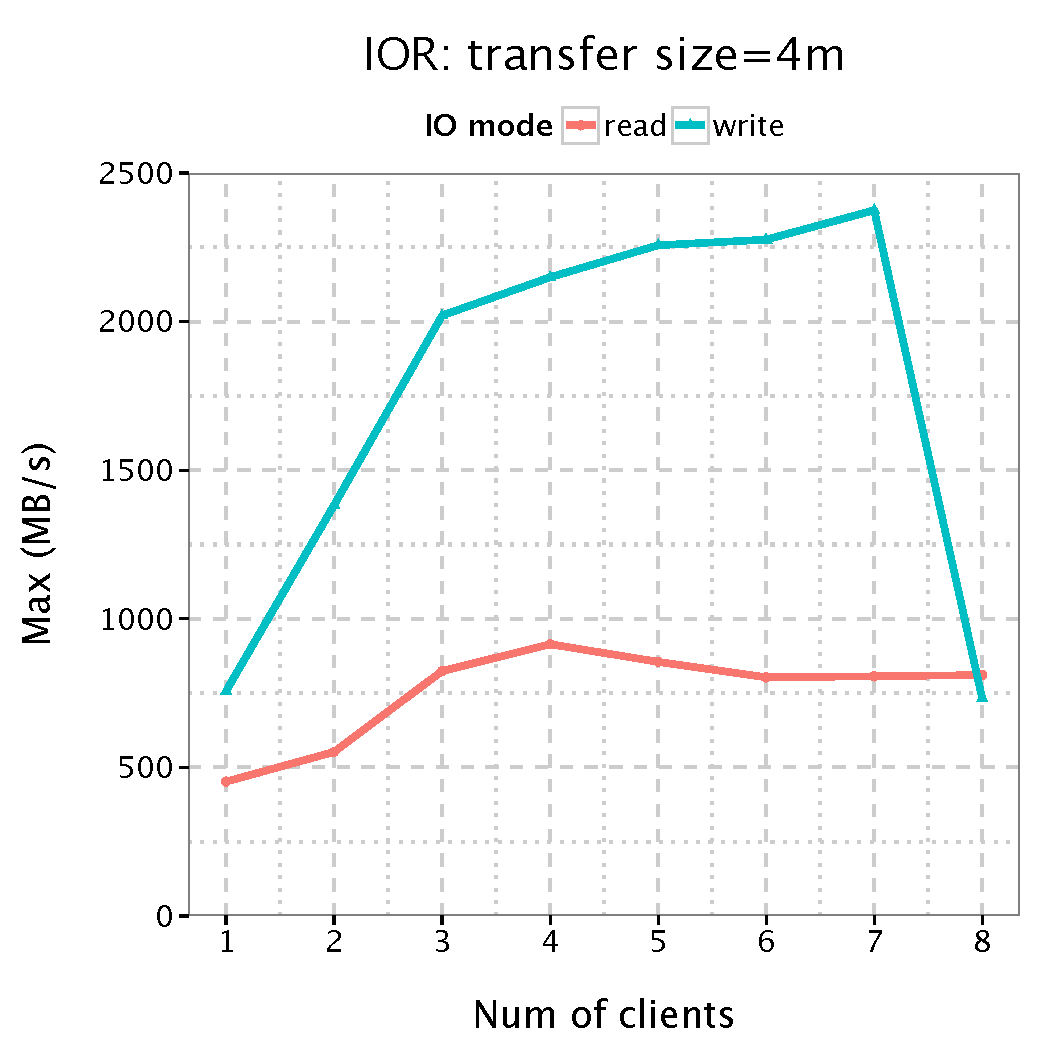
\includegraphics[width=3in]{data/ior_4m}
\label{fig:ior4m}}
}% end of centerline
\caption{CephFS scalability test with IOR}

\end{figure*}


\begin{itemize}

  \item The small read (4 KB transfer size) performance is almost an anomaly
  -- we will investigate why it is so low compare to write performance and
  present improved results in Section~\ref{sec:improve-ior}.

  \item The large read (4 MB transfer size) performance is almost half of the
  RADOS read performance.
   
  \item The write performance is also about half of what we can obtain from
  RADOS Bench. When number of clients reaches 8, there is a significant
  performance drop as well. 

\end{itemize}


We will describe the efforts and results on performance improvement in the
following sections.


\section{Further Optimization \\and Improvements}
\label{sec:ceph-tuning}

\subsection{Improving RADOS Performance}

\begin{figure}[h]
\centering
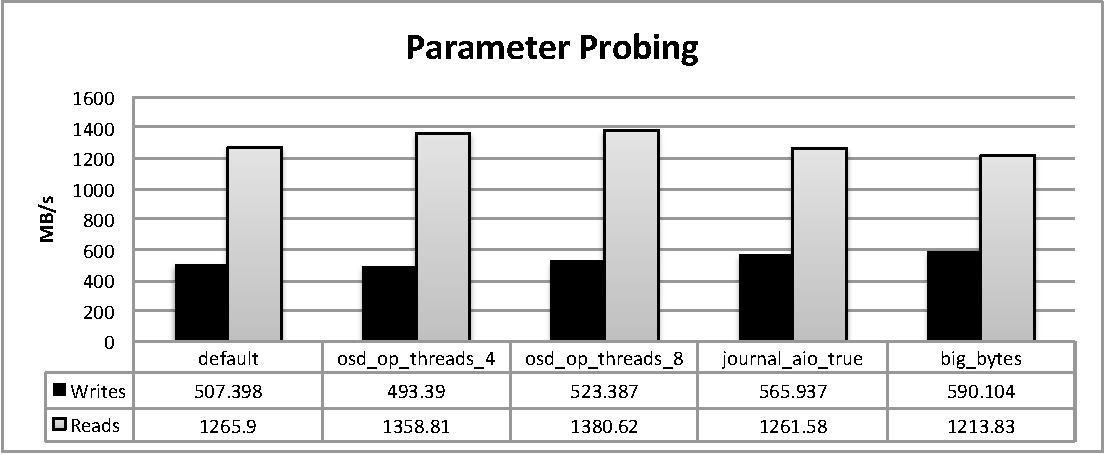
\includegraphics[width=3.5in]{para2}
%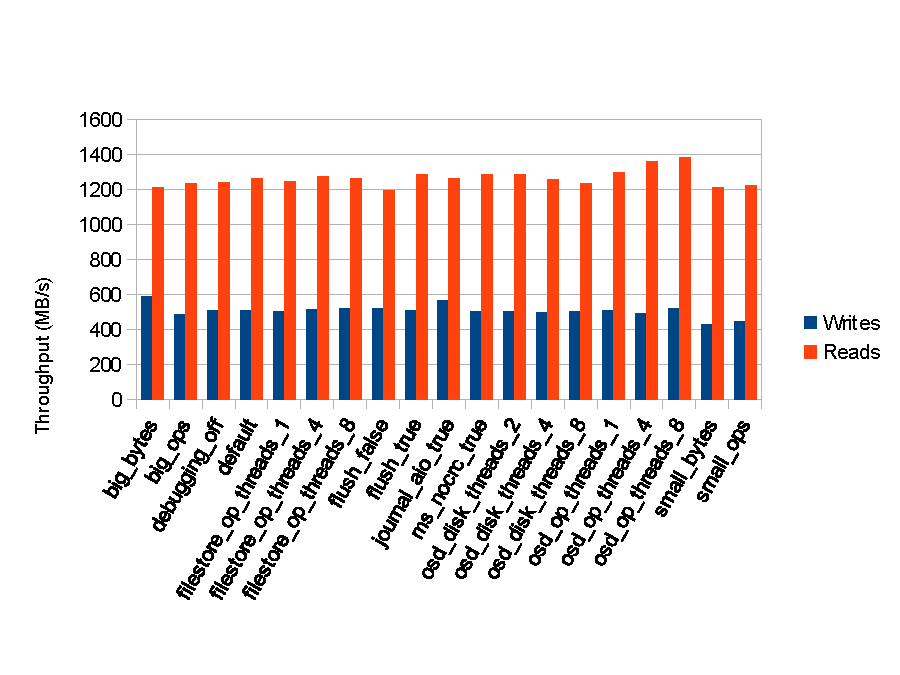
\includegraphics[width=3.5in]{parametric}
\caption{Evaluating parameter impact through sweeping test}
\label{fig:parametric}
\end{figure}

After the initial test results, we tried various combinations of tweaks
including: changing the number of filestore op threads, putting all of the
journals on the same disks as the data, doubling the OSD count, and upgrading
Ceph to a development version which reduces the seek overhead caused by
\texttt{pginfo} and \texttt{pglog} updates on XFS (these enhancements are now
included as of the Ceph Cuttlefish release, v0.61).  

%The two biggest
%improvements resulted from disabling CRC32c checksums and increasing the OSD
%count on the server.  With these changes, we are seeing better results.

We swept over Ceph configuration parameters to examine how different tuning
options affect performance on the DDN platform. The result of this parameter
probing is illustrated in Figure~\ref{fig:parametric}. Please refer to
Appendix E of \cite{ceph:techreport} for explanations of these probed
parameters. In this figure, the default is where we started with. Reads
benefit from increasing the \verb!osd_op_threads! (4 and 8), with 7.3\% and
9\% improvement respectively. For writes, the substantial boost comes with
\verb!journal_aio! true and \verb!big_bytes!, with 11.5\% and 16.3\%
improvement respectively. Other probed parameters (not shown on this figure)
doesn't bear tangible impacts.


%As a result of this testing, we improved performance slightly by
%increasing the size of various Ceph buffers and queues, enabling AIO journals,
%and increasing the number of OSD op threads.

\begin{comment}

\subsubsection{Disable Cache Mirroring on Controllers}

During a second round of test performed by Inktank, we noticed a dramatic drop
on RADOS performance: even though write throughput on individual server met the
expectation, it did not scale across servers.

We spent a significant amount of time
investigating this phenomenon. Ultimately, we were able to replicate this finding
when running concurrent disk throughput tests directly on the servers without
Ceph involved. The second RAID processor on each DDN controller would max out when
three or more LUNs were written concurrently. It turns out the root of the problem
was a regression on DDN firmware update -- in particular, the cache
mirroring was not behaving as it should.\footnote{DDN recently released a new
firmware version and we were told the issue has been fixed. Unfortunately, we didn't get
a chance to verify it during our test cycle.}

%% SCOTT - is running with cache mirroring off and option for a production system or not?
%% What are the consequences? Did DDN eventually provide a fix? If yes, were we able to test
%% with it or not?

%% FEIYI: add footnote to clarify the issue.

\begin{figure}[htb]
\centering
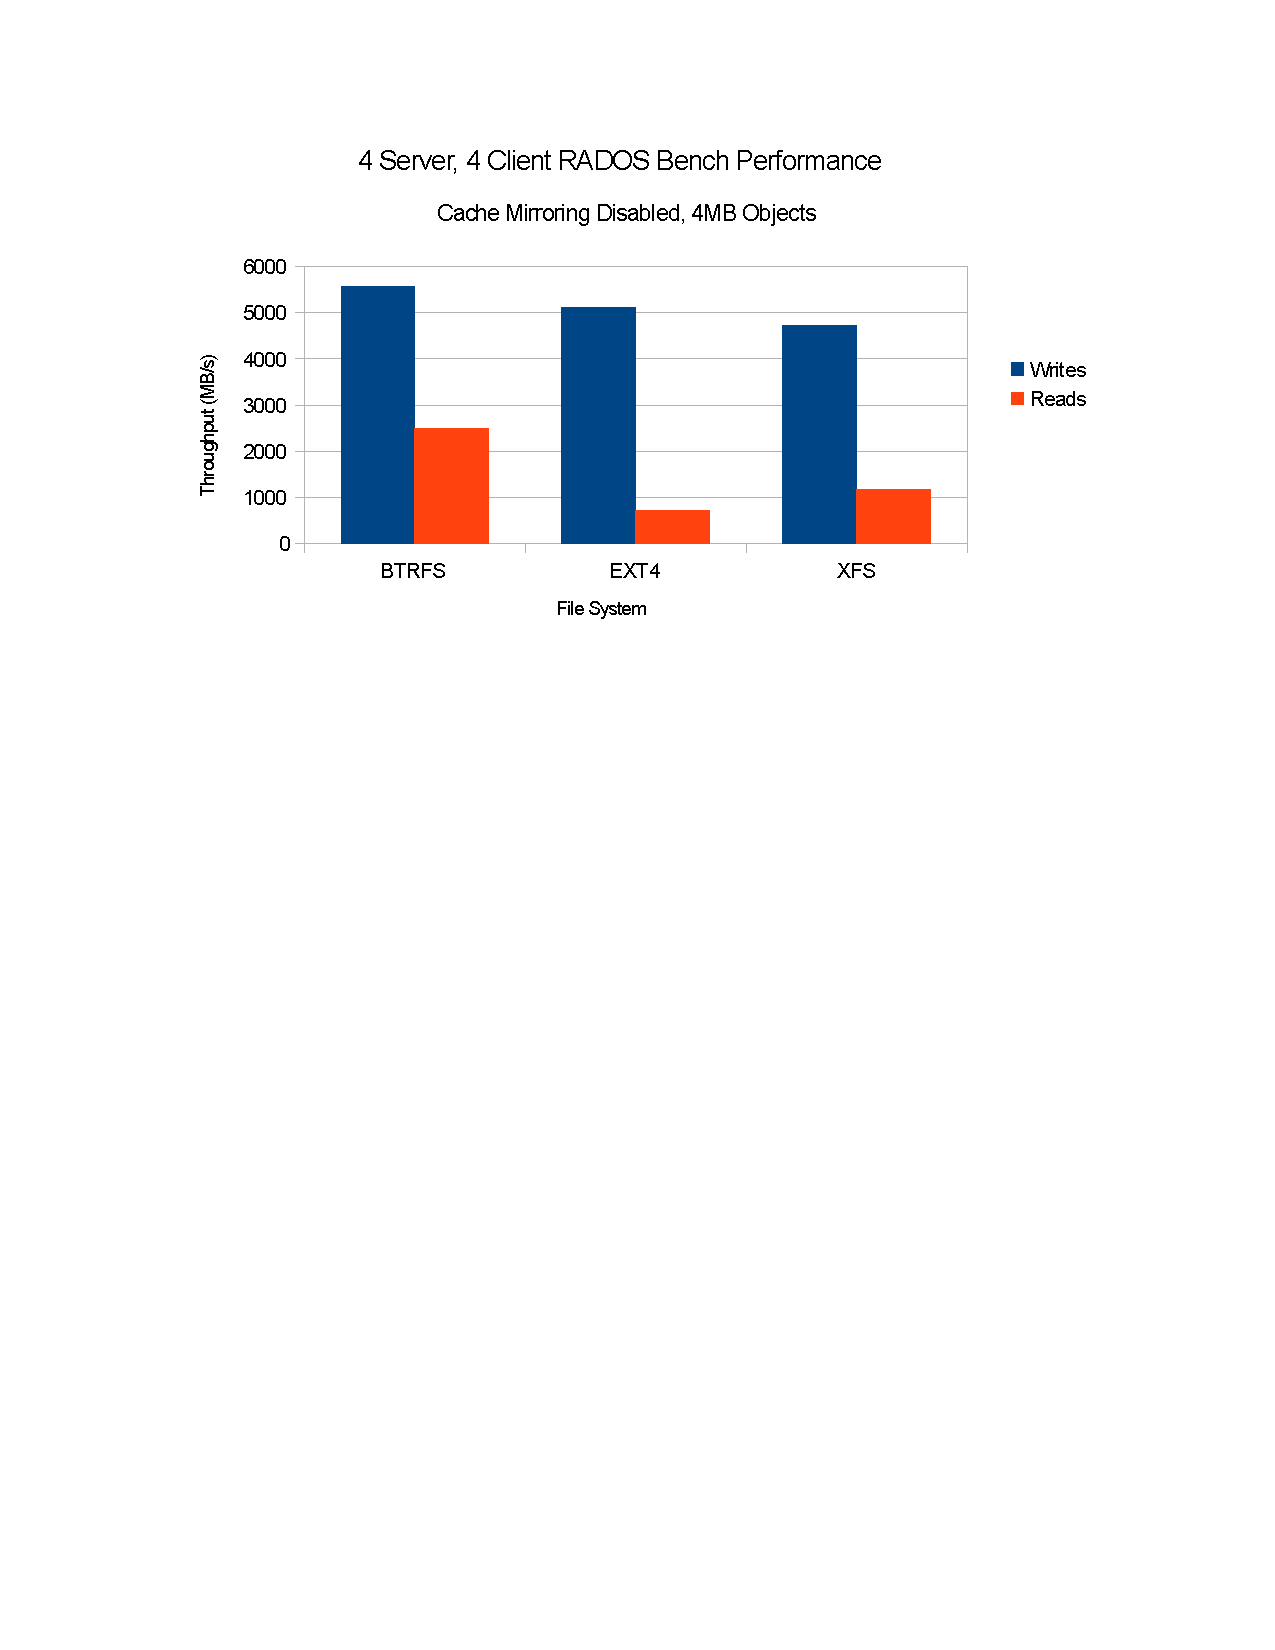
\includegraphics[width=3.5in]{rados-after-ddn}
\caption{Evaluating RADOS bench after disabling cache mirroring}
\label{fig:rados-ddn-mirror-disabled}
\end{figure}


With cache mirroring disabled, write performance when using all four servers
improved dramatically, as illustrated in
Figure~\ref{fig:rados-ddn-mirror-disabled}. With BTRFS, for example, we hit over
5.5 GB/s from the clients.  When accounting for journal writes, that is over
11 GB/s to the disks and very close to what the DDN chassis is capable of doing. 
Unfortunately, read performance did not scale as well.


\subsubsection{Repeating RADOS Scaling Test}

We now repeated the previous RADOS scaling tests with these improvements in place.
The first test was done on a single node with RADOS Bench to see how close the
underlying object store could get to the node hardware limitations as the number
of OSDs/LUNs used on the node increased. All the tests performed were against
XFS-formatted storage.

%% SCOTT - the title in the figure needs to change IO to I/O

%% SCOTT - how do writes inc. journals exceed the client network max? Dual ports
%% on the single server?

\begin{figure}[htb]
\centering
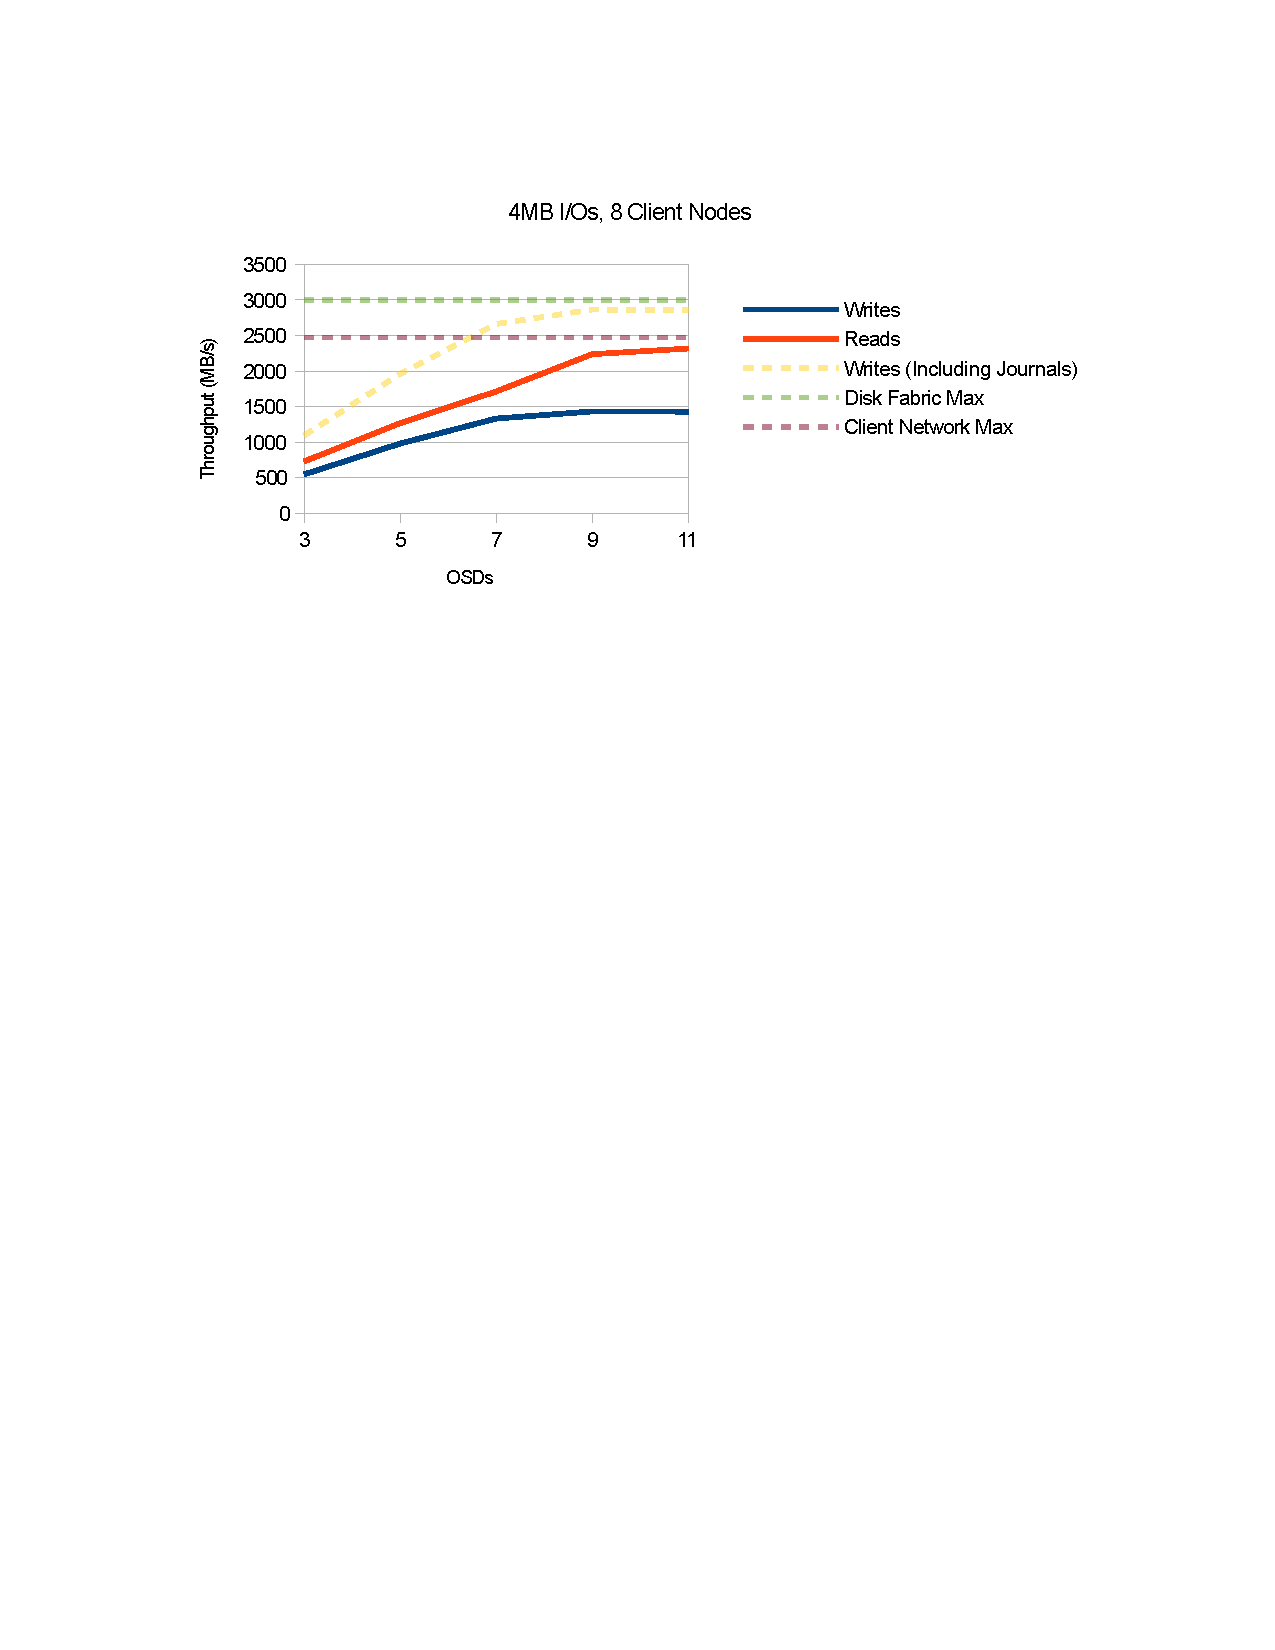
\includegraphics[width=3.5in]{rados-064-osd}
\caption{RADOS Bench Scaling on number of OSD, Ceph 0.64, 4 MB I/O, 8 Client Nodes}
\label{fig:rados-064-osd}
\end{figure}

In the single server case as shown in Figure~\ref{fig:rados-064-osd}, ``Writes
(including Journals)'' refers to how much data is actually being written out
the DDN SFA10K (observed directly from the controllers), and blue line is how
much data the clients are writing.  We observe that performance observed by the
DDN controllers gets very close to the hardware limits at roughly 9 OSDs per
server and then mostly levels out.

We also repeated tests looking at RADOS Bench performance as the number of OSD
server nodes increases from one to four. The results are summarized in
Figure~\ref{fig:rados-064-oss}. As the number of nodes increases, performance
scales nearly linearly for both reads and writes.

%% SCOTT - why does the client network max scale in figure 12 but not figure 11?
%% Do they no measure the same thing (i.e. a single server)? If not, the text
%% needs to make it more clear.

\begin{figure}[htb]
\centering
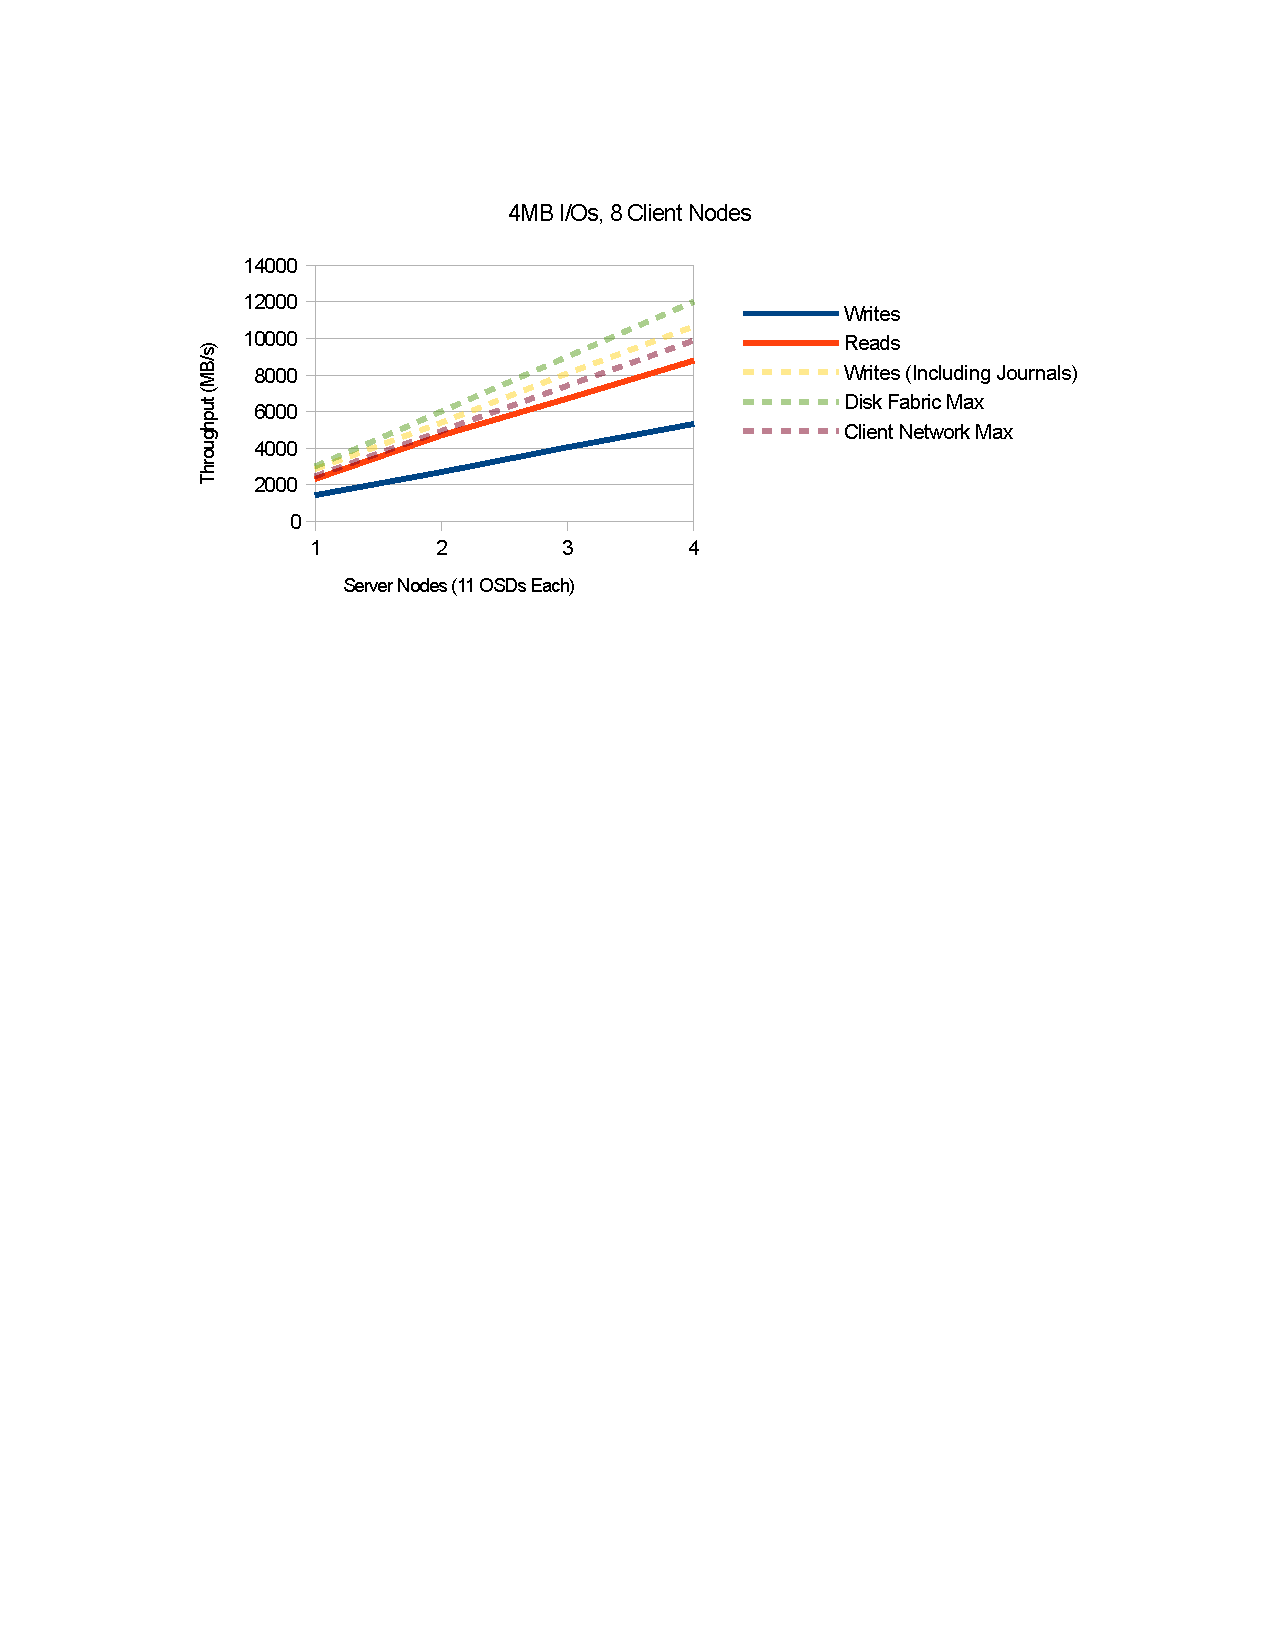
\includegraphics[width=3.5in]{rados-064-oss}
\caption{RADOS Bench Scaling on number of servers, Ceph 0.64, 4 MB I/O, 8 client
nodes}
\label{fig:rados-064-oss}
\end{figure}

\end{comment}



\subsection{Improving Ceph File System Performance}
\label{sec:ceph-tuning-fs}

The initial stability issues mentioned in Section~\ref{sec:ior-initial} are
fixed by migrating from Ceph version 0.48/0.55 to 0.64, the latest stable
version at the time of writing this report.  Upgrading to the latest stable
Ceph release allowed us to run a full IOR parameter sweep for the first time
since we started evaluating the performance and scalability of the Ceph file
system.  This is another sign of how much Ceph development is currently in
flux.

%%%%%%%%%%%%%%%%%%%%%%%%%%%%%%%%%%% removed for space

\begin{comment}

Another fix introduced by Ceph version 0.64 was in pool creation.  The default
data pool used by previous Ceph version were set to 2x replication by mistake.
This potentially halved the write performance. With version 0.64 we explicitly
set the replication level to 1, which is the preferred value for a HPC
environment like ours running on high-end and reliable storage backend hardware
(e.g. DDN SFA10K).

\end{comment}


Even with these changes in place, less-than-ideal write performance and very
poor read performances were observed during our tests.  We also observed that
by increasing the number of IOR processes per client node, the read
performance degraded even further indicating some kind of contention either on
the clients or on the OSD servers.


\subsubsection{Disabling Client CRC32}

At this point, we were able to both make more client nodes available for Ceph
file system-level testing and also install a profiling tool called \verb!perf!
that is extremely useful for profiling both kernel and user space codes.
Profiling with \verb!perf! showed high CPU utilization on test clients due to
CRC32c processing in the Ceph kernel client.  

%%%%%%%%%%%%%%%%%%%%%%%%%%%%%%%%%% removed

%CRC32 checksums can be disabled
%by changing the CephFS mount options:

%\begin{Verbatim}[fontsize=\small]
%mount -t ceph 10.37.248.43:6789:/ 
%    /mnt/ceph -o name=admin,nocrc
%\end{Verbatim}


With client CRC32 disabled, we repeated the IOR tests. New results are shown in
in Figure~\ref{fig:ior-no-client-crc32}. 

\begin{figure}[htb]
\centering
%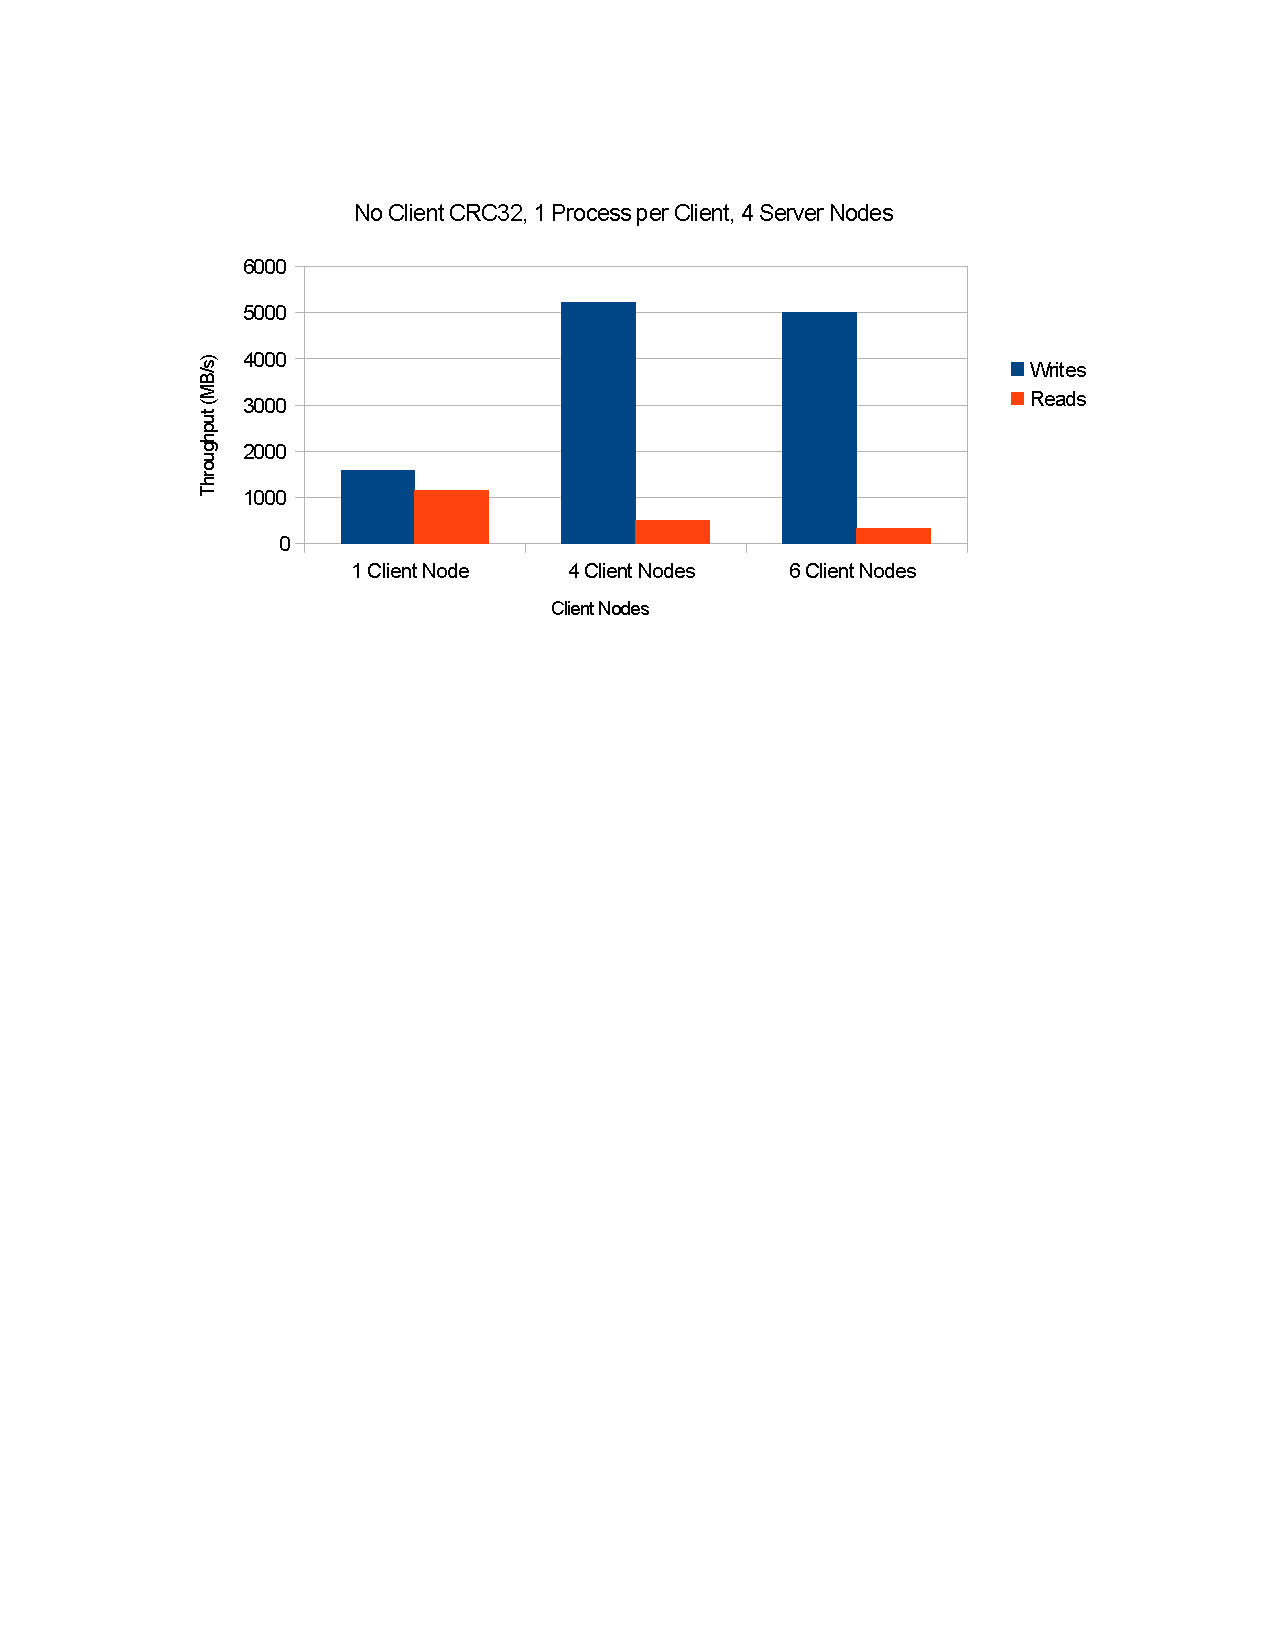
\includegraphics[width=3.5in]{ior-client-no-crc32}
%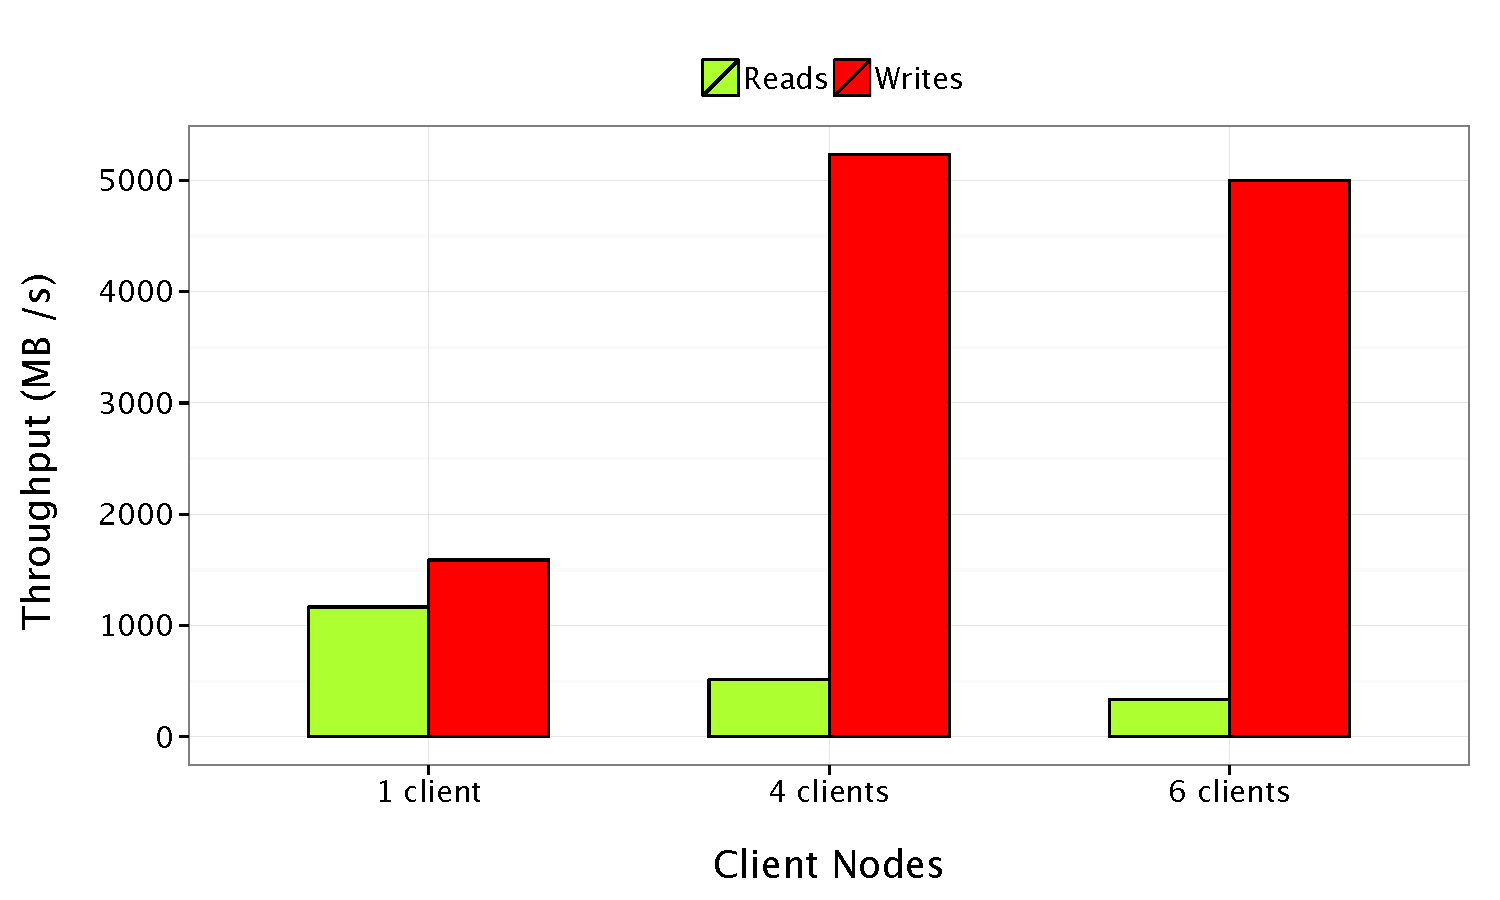
\includegraphics[width=3.5in]{ior_no_crc}
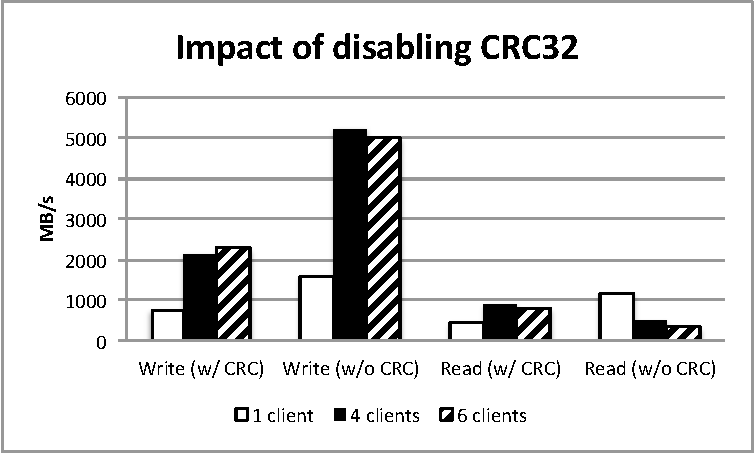
\includegraphics[width=3.5in]{crc32}
\caption{Impact of Disabling CRC32}
\label{fig:ior-no-client-crc32}
\end{figure}

We observed that IOR write throughput increased dramatically and is now very
close and comparable to the RADOS Bench performance. Read performance continued
to be poor and continued to scale inversely with the increasing number of
client processes.  Please note that, since these tests were performed, Inktank
has implemented SSE4-based CRC32 code for Intel CPUs.  While any kernel based
CRC32 processing should have already been using SSE4 instructions on Intel
CPUs, this update will allow any user-land Ceph processes to process CRC32
checksums with significantly less overhead.

\subsubsection{Improving IOR Read Performance}

Deeper analysis with \verb!perf! showed that there was heavy lock contention
during parallel compaction in the Linux kernel memory manager.  This behavior
was first observed roughly in the kernel 3.5 time frame which was the kernel
installed on our test systems.\footnote{For more information,
please refer to \url{http://lwn.net/Articles/517082/} and
\url{https://patchwork.kernel.org/patch/1338691/}.}  We upgraded our test
systems with kernel version 3.9 and performed RADOS Bench test.  The results
%were dramatic:  read performance improved from 4678 MB/s to 8643 MB/s (almost
were dramatic:  read performance improved from 4678 MB/s to 7499 MB/s 
(a 60\% improvement).  Write performance was also fractionally improved from
4720 MB/s to 5284 MB/s (a 12\% improvement).
%extremely positive and presented in
%Figure~\ref{fig:rados-kernel}. As can be seen, with the 3.9 kernel, while
%there was a slight improvement on write performance, read performance improved
%dramatically.  In addition to the kernel change, the amount of CephFS client
%kernel read-ahead cache size was increased as well.


%\begin{figure}[htb]
%\centering
%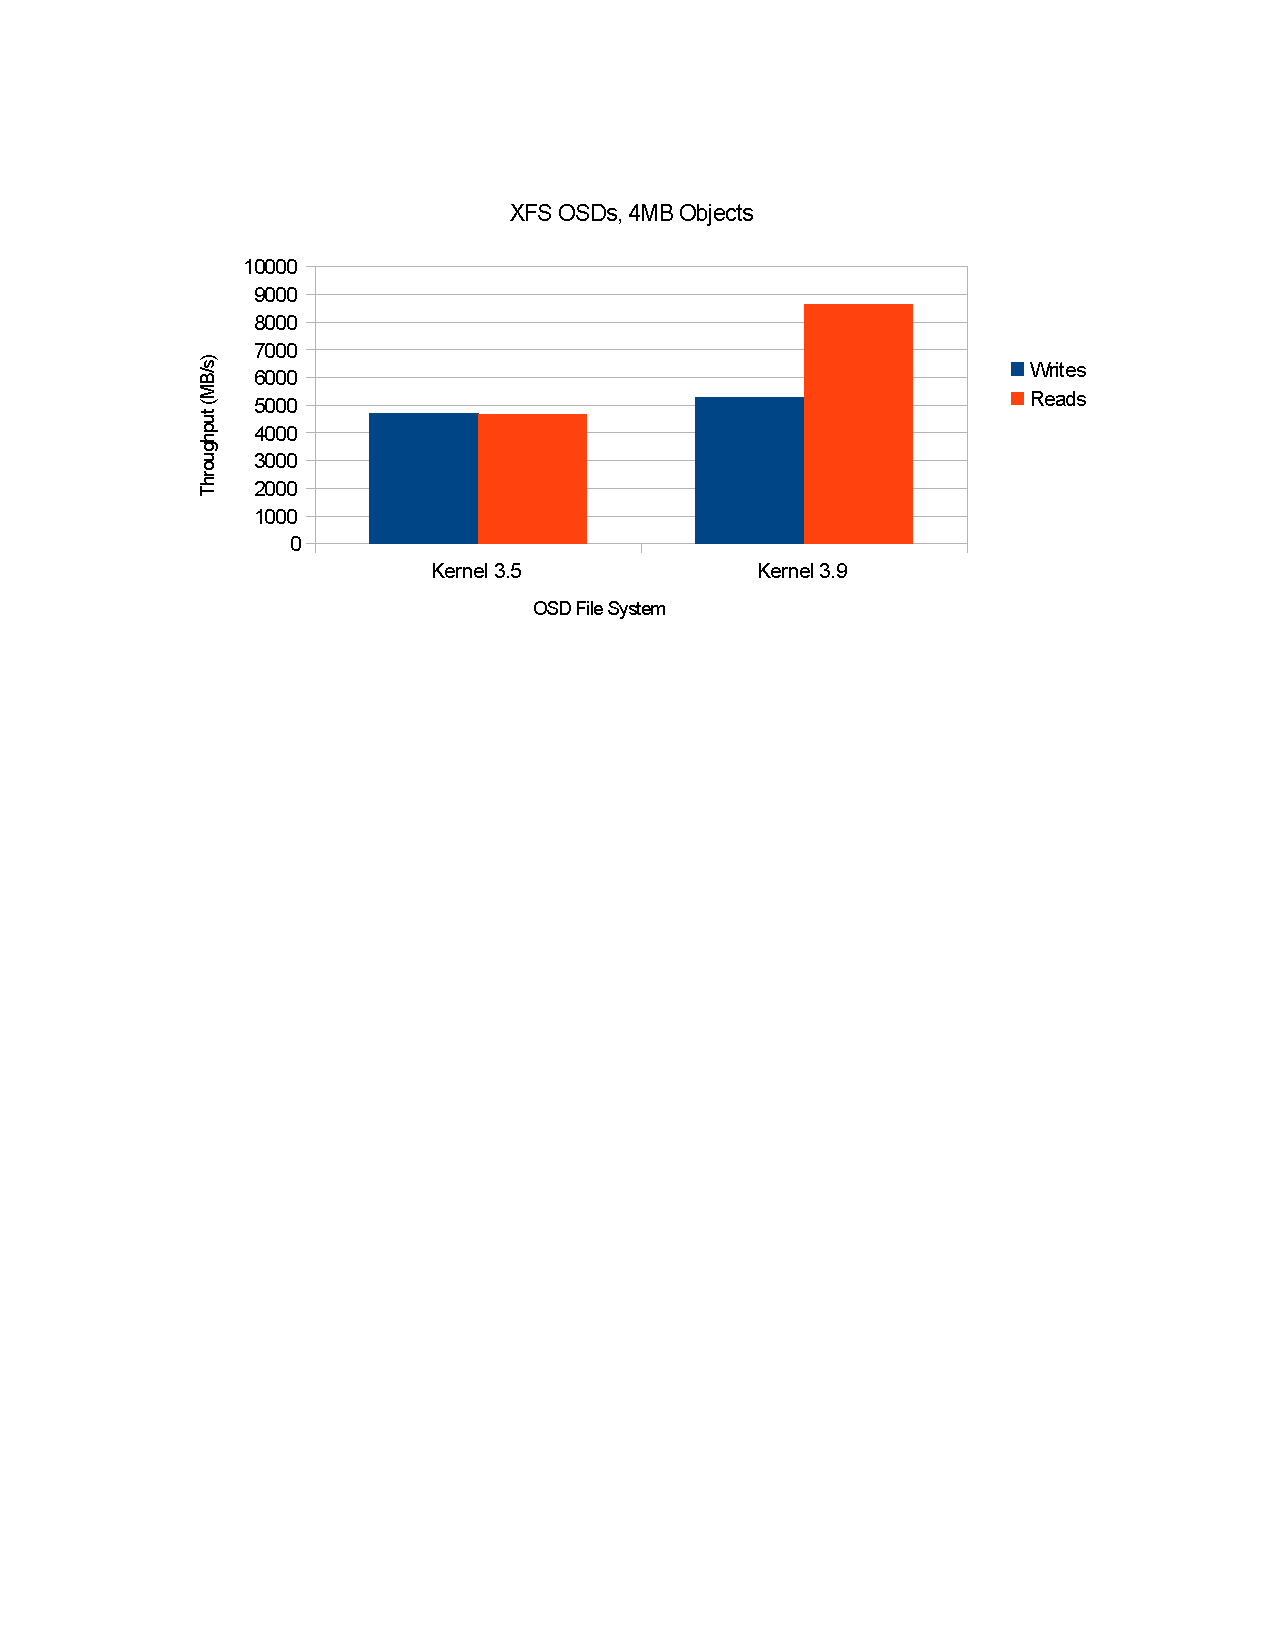
\includegraphics[width=3.5in]{rados-kernel-35vs39}
%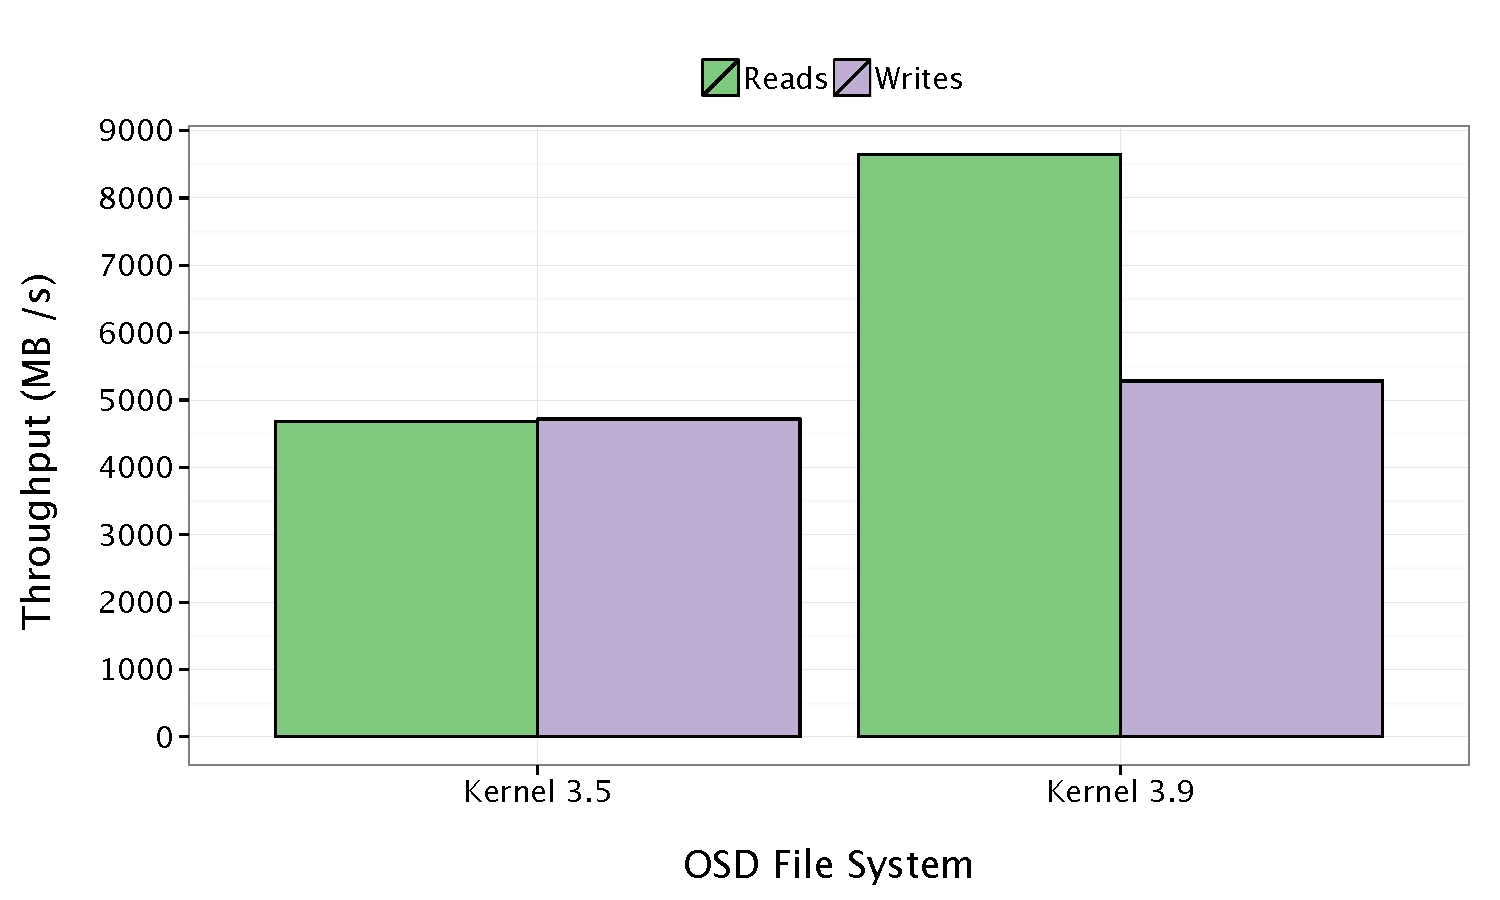
\includegraphics[width=3.5in]{rados_kernel}
%\caption{RADOS bench: Linux kernel version 3.5 vs. 3.9}
%\label{fig:rados-kernel}
%\end{figure}



%%%%%%%%%%%%%%%%%%%%%%%%%%%% REMOVED to save space

%\begin{Verbatim}[samepage=true, fontsize=\small]
%mount -t ceph 10.37.248.43:6789:/ 
%  /mnt/ceph -o name=admin,nocrc,
%  readdir_max_bytes=4104304,
%  readdir_max_entries=8192
% \end{Verbatim}

%% SCOTT - is figure 15 IOR over Ceph and 14 is RADOS bench? If so, can we
%% mention that 15 shows the filesystem performance?

Additionally, we increased the size of the CephFS kernel client's read-ahead
cache.  
%IOR results reflecting the read-ahead cache size change are presented in
%Figure~\ref{fig:ior-kernel-39}.

\begin{comment}
\begin{figure}[htb]
\centering
%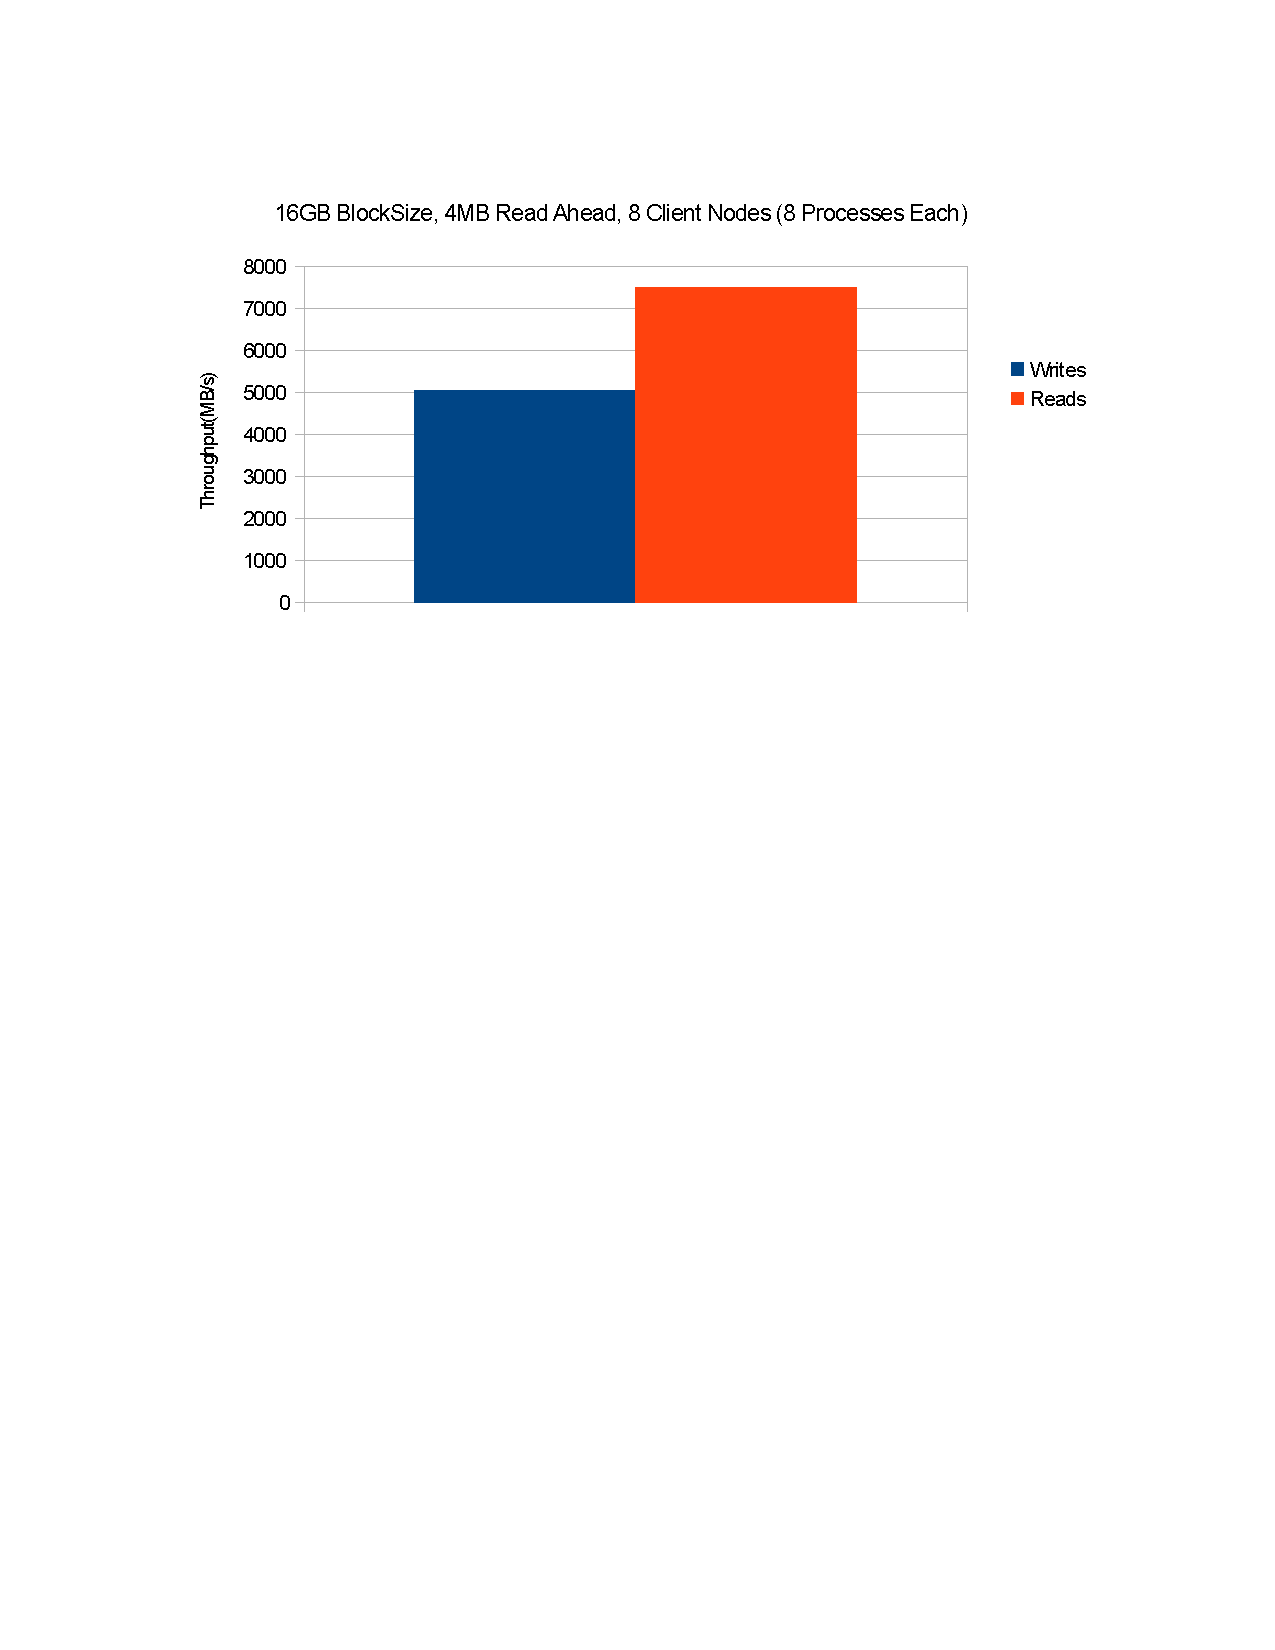
\includegraphics[width=3.5in]{ior-kernel-39}
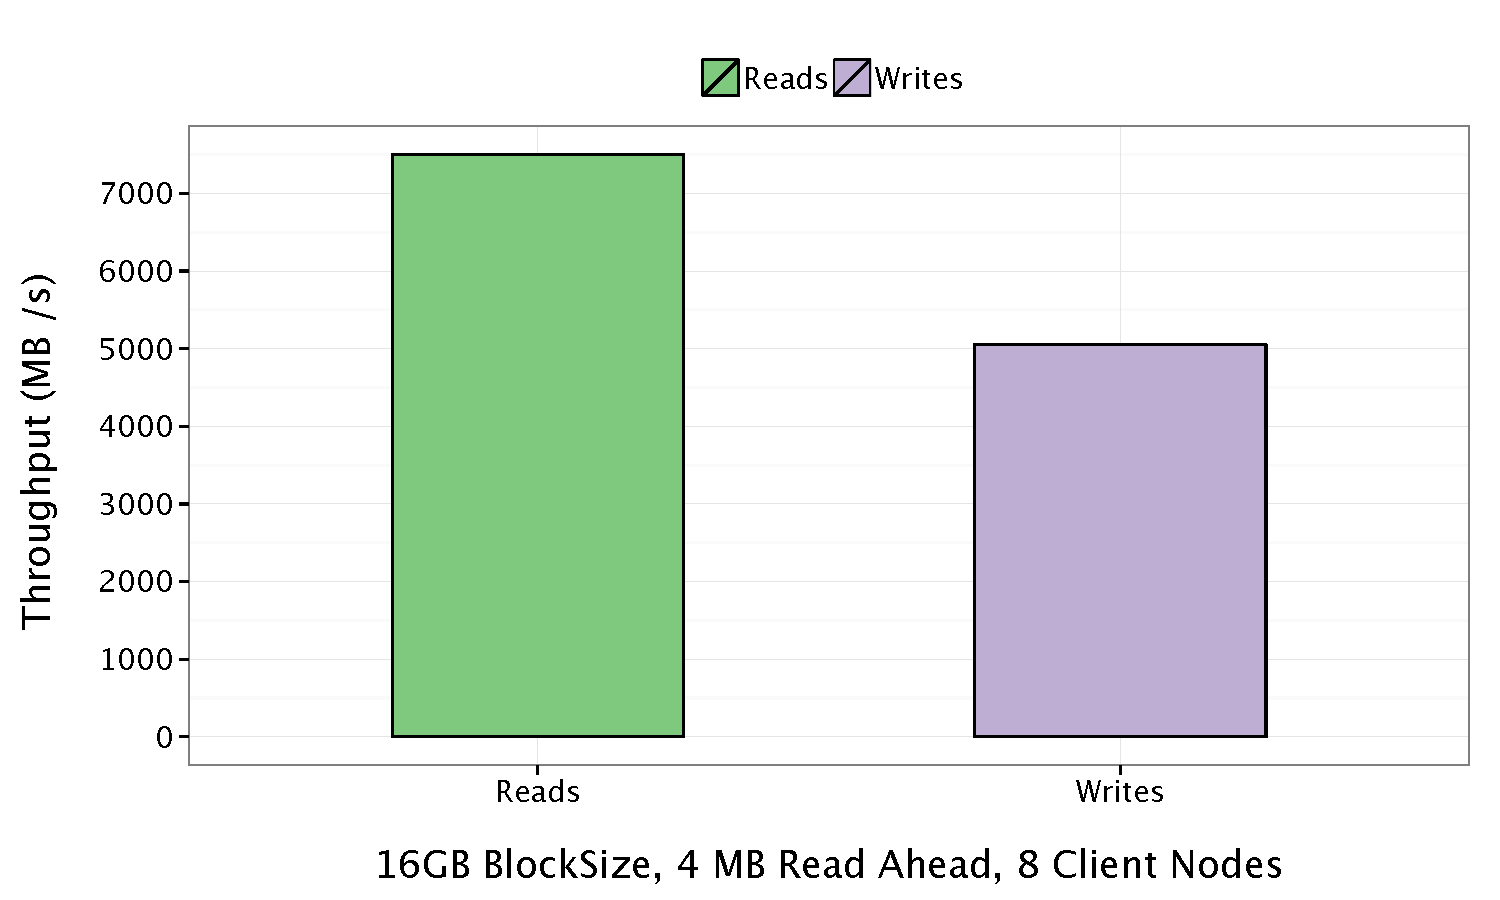
\includegraphics[width=3.5in]{ior_kernel_change}
\caption{CephFS performance with kernel changes to 3.9, IOR with 4 MB transfer
size}
\label{fig:ior-kernel-39}
\end{figure}
\end{comment}

By installing a newer kernel, increasing read-ahead cache size, and increasing
the number of client IOR processes, we were able to achieve very satisfactory
I/O performance at the Ceph file system-level.


\subsubsection{Repeating the IOR Scaling Test}

As before, we ran IOR scaling tests with two cases: transfer size 4 KB and 4
MB.  These results are illustrated in Figure~\ref{fig:ior-064}, respectively.
As expected, we saw saw  improved read and write performance. These new read
and write performance are in line with observed RADOS bench performance.

%% SCOTT - Can we use the same Y axis for these figures? Any comment from Inktank
%% as to why 4 KB performance is better than 4 MB performance?

\begin{figure}[htb]
\centering
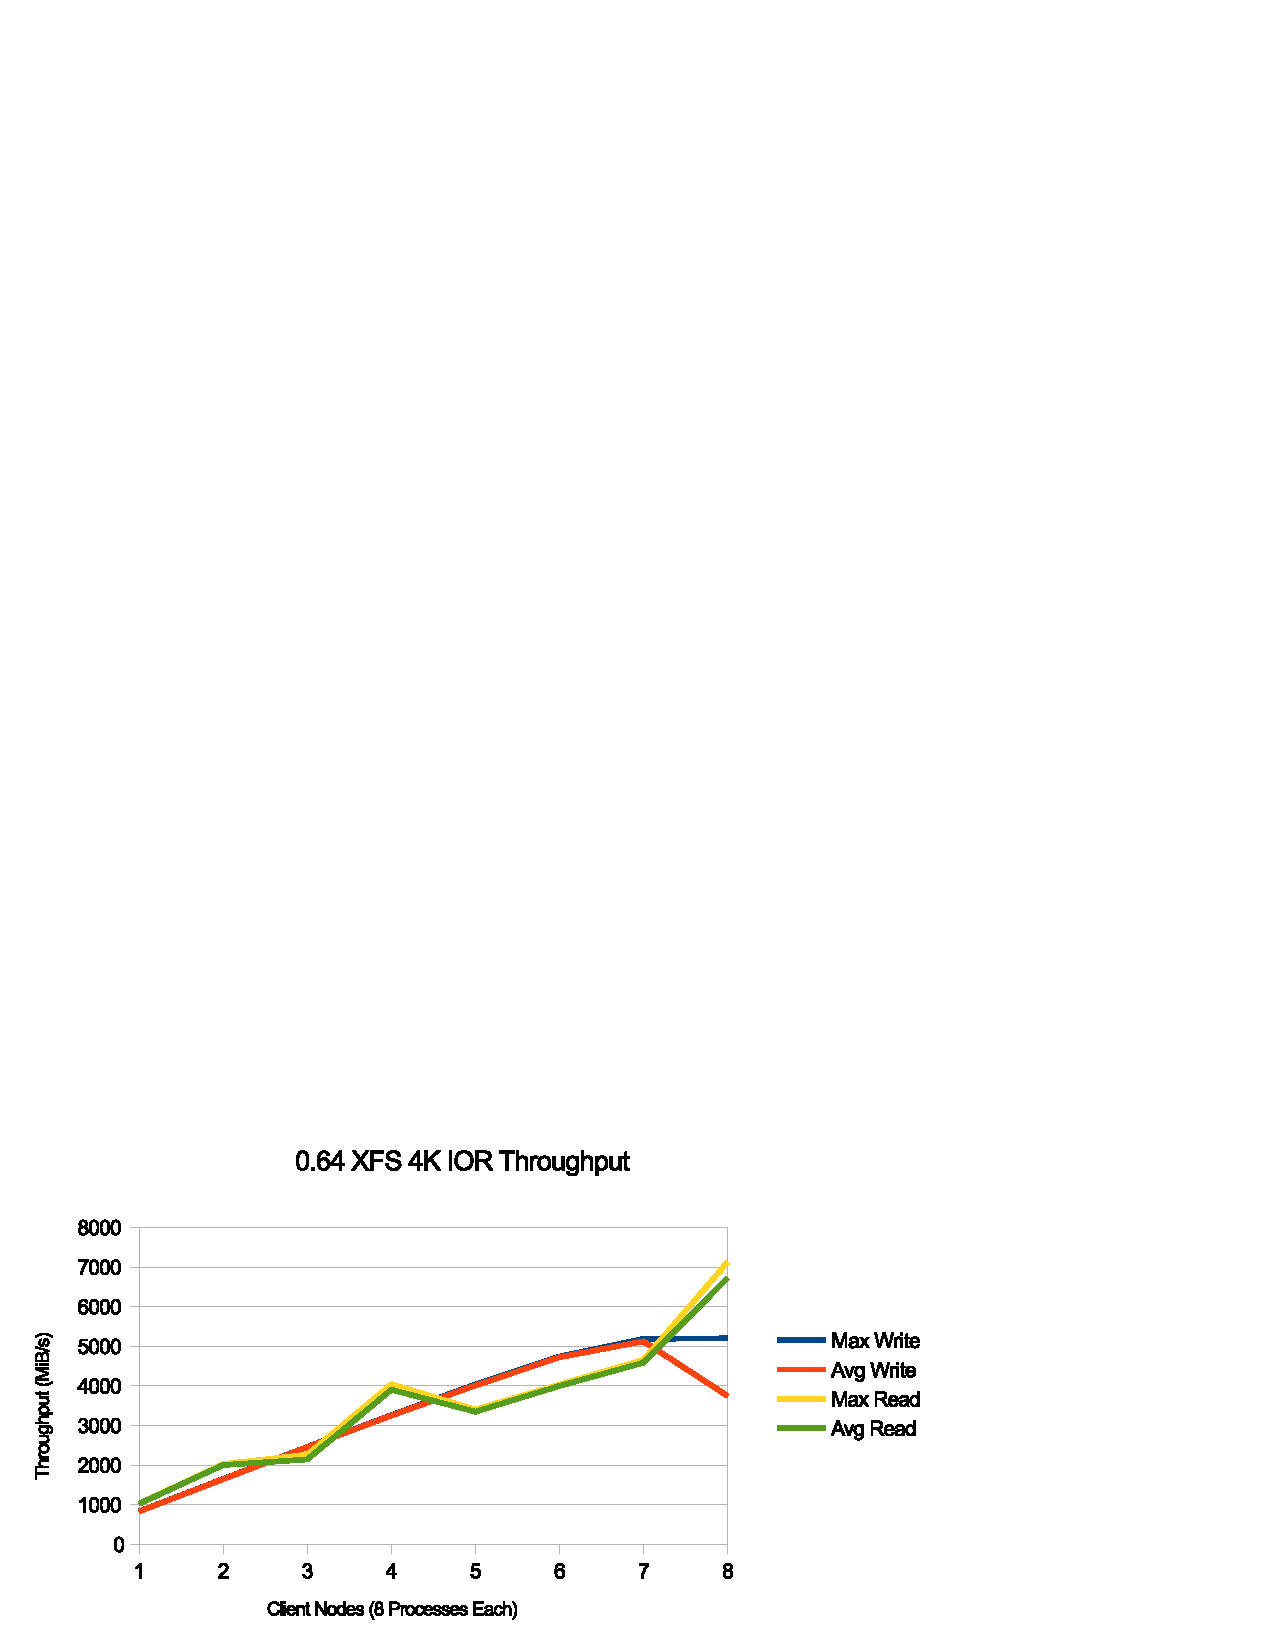
\includegraphics[width=3.5in]{ior-064-4k}
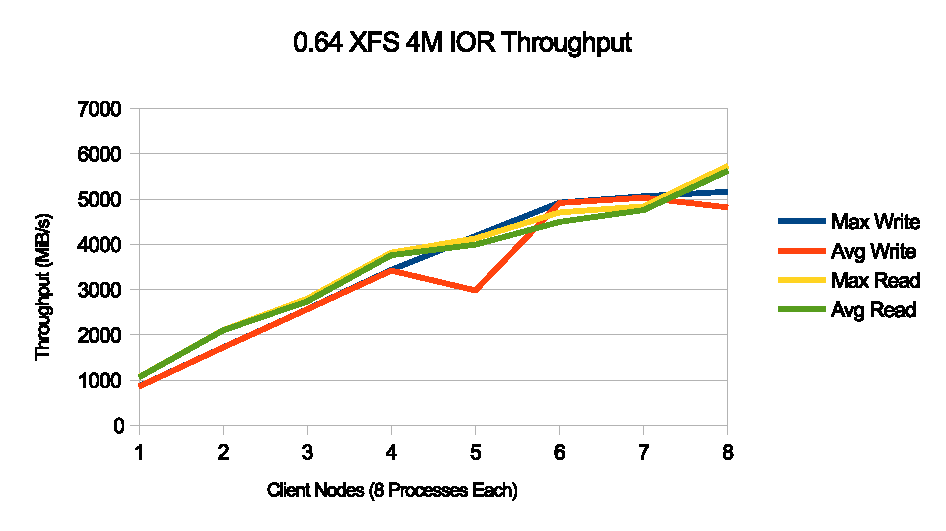
\includegraphics[width=3.5in]{ior-064-4m}
\caption{IOR Scaling Test: 4 KB and 4 MB transfer size}
\label{fig:ior-064}
\end{figure}

Throughout our IOR testing, we observed that the average write throughput is
lower than the maximum.  This behavior was observed during other tests as well,
indicating that we may have periods of time where write throughput is
temporarily degrading.  Despite these issues, performance generally seems to be
improving with respect to increasing number of clients.  Writes seem to be
topping out at around 5.2 GB/s (which is roughly what we would expect due to
journalling effectively halving the write performance).  Reads seem to be
topping out anywhere from 5.6-7 GB/s, however it is unclear if read performance
would continue scaling with more clients and get closer to ~8 GB/s we observed 
with RADOS Bench.

\begin{comment}
\subsection{Metadata Performance Tuning}
For brevity's sake, we are omitting most of our file and directory creation
rate results.  However, over the course of our testing we did notice that in
CephFS 0.64 a significant improvement in the performance of file creation with
mdtest.  Shown in Figure~\ref{fig:mdtest-064-file-create}, we note
that as number of clients increase, the file creation rate does not scale
linearly, which suggested some form of lock contention.  Due to the large
differences in the initially observed performance, and the performance with
Ceph 0.64, opportunities for file and directory create tuning may be
substantial. 

\begin{figure}[htb]
\centering
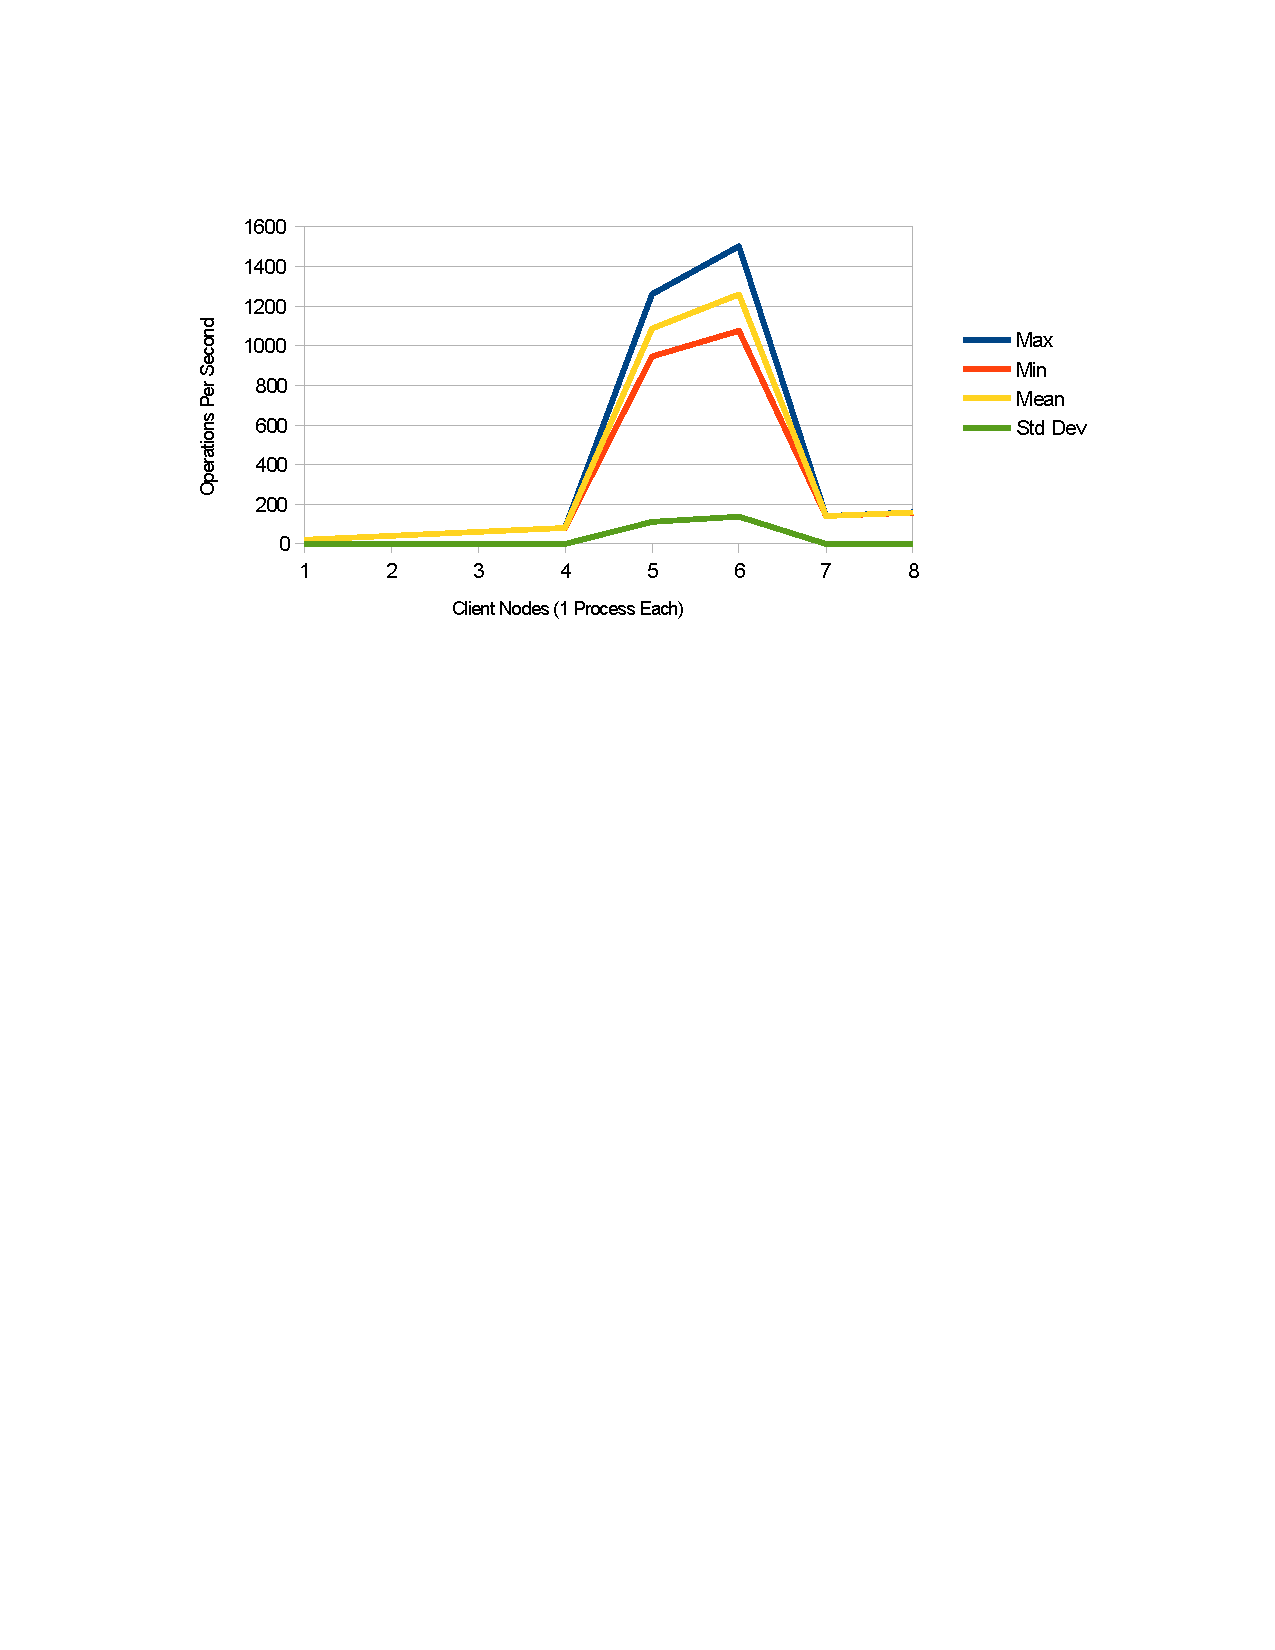
\includegraphics[width=3.5in]{mdtest-064-file-create}
\caption{mdtest of file creation on Ceph 0.64}
\label{fig:mdtest-064-file-create}
\end{figure}

\end{comment}

\section{Observations and Conclusions}
\label{sec:conclusion}

Ceph is built on the assumption that the underlying hardware components
are unreliable, with little or no redundancy and failure detection capability.
This assumption is not valid for high-end HPC centers like ours. We have
disabled replication for pools, we haven't measured and quantified
processing overhead and we do not know yet if this would be significant.

Ceph performs \textbf{metadata + data} journaling, which is fine for host
systems that have locally attached disks. However, this presents a problem in
DDN SFA10K-like hardware, where the backend LUNs are exposed as block devices
through IB over SRP protocol. The journaling write requires twice the
bandwidth compared to Lustre-like meta data-only journaling mechanism. For
Ceph to be viable in large-scale capability HPC environments like ours,
journaling operations will need further design and more engineering efforts.

In our earlier tests, we experienced large performance swings during different
runs, low read performance when transfer size is small, and I/O errors tend to
happen when system is under stress (more clients and large transfer sizes).
However, with systematic performance engineering and development efforts, we
have seen a steady improvement through different releases. As of now, Ceph
system on our testbed is able to perform close to 80\% of raw hardware
capability at RADOS level and close to 70\% at file system level. This is
still no comparison to Lustre yet, but by no means a small feat for such a
\textit{young} technology. It is, in fact, a very respectable level of
performance. 

%The current design on journaling write does present a challenge in
%our IB-switched storage hardware. As BTRFS and other backend file system
%mature, we are seeing promising signs for Ceph to take advantage for a
%better journaling design.






% An example of a floating figure using the graphicx package.
% Note that \label must occur AFTER (or within) \caption.
% For figures, \caption should occur after the \includegraphics.
% Note that IEEEtran v1.7 and later has special internal code that
% is designed to preserve the operation of \label within \caption
% even when the captionsoff option is in effect. However, because
% of issues like this, it may be the safest practice to put all your
% \label just after \caption rather than within \caption{}.
%
% Reminder: the "draftcls" or "draftclsnofoot", not "draft", class
% option should be used if it is desired that the figures are to be
% displayed while in draft mode.
%
%\begin{figure}[!t]
%\centering
%\includegraphics[width=2.5in]{myfigure}
% where an .eps filename suffix will be assumed under latex, 
% and a .pdf suffix will be assumed for pdflatex; or what has been declared
% via \DeclareGraphicsExtensions.
%\caption{Simulation Results}
%\label{fig_sim}
%\end{figure}

% Note that IEEE typically puts floats only at the top, even when this
% results in a large percentage of a column being occupied by floats.


% An example of a double column floating figure using two subfigures.
% (The subfig.sty package must be loaded for this to work.)
% The subfigure \label commands are set within each subfloat command, the
% \label for the overall figure must come after \caption.
% \hfil must be used as a separator to get equal spacing.
% The subfigure.sty package works much the same way, except \subfigure is
% used instead of \subfloat.
%
%\begin{figure*}[!t]
%\centerline{\subfloat[Case I]\includegraphics[width=2.5in]{subfigcase1}%
%\label{fig_first_case}}
%\hfil
%\subfloat[Case II]{\includegraphics[width=2.5in]{subfigcase2}%
%\label{fig_second_case}}}
%\caption{Simulation results}
%\label{fig_sim}
%\end{figure*}
%
% Note that often IEEE papers with subfigures do not employ subfigure
% captions (using the optional argument to \subfloat), but instead will
% reference/describe all of them (a), (b), etc., within the main caption.


% An example of a floating table. Note that, for IEEE style tables, the 
% \caption command should come BEFORE the table. Table text will default to
% \footnotesize as IEEE normally uses this smaller font for tables.
% The \label must come after \caption as always.
%
%\begin{table}[!t]
%% increase table row spacing, adjust to taste
%\renewcommand{\arraystretch}{1.3}
% if using array.sty, it might be a good idea to tweak the value of
% \extrarowheight as needed to properly center the text within the cells
%\caption{An Example of a Table}
%\label{table_example}
%\centering
%% Some packages, such as MDW tools, offer better commands for making tables
%% than the plain LaTeX2e tabular which is used here.
%\begin{tabular}{|c||c|}
%\hline
%One & Two\\
%\hline
%Three & Four\\
%\hline
%\end{tabular}
%\end{table}


% Note that IEEE does not put floats in the very first column - or typically
% anywhere on the first page for that matter. Also, in-text middle ("here")
% positioning is not used. Most IEEE journals/conferences use top floats
% exclusively. Note that, LaTeX2e, unlike IEEE journals/conferences, places
% footnotes above bottom floats. This can be corrected via the \fnbelowfloat
% command of the stfloats package.







% use section* for acknowledgement
\section*{Acknowledgment}

The authors would like to thank Galen Shipman of ORNL for initiating the
evaluation effort, and Greg Farnum of Inktank for providing early support.


% trigger a \newpage just before the given reference
% number - used to balance the columns on the last page
% adjust value as needed - may need to be readjusted if
% the document is modified later
%\IEEEtriggeratref{8}
% The "triggered" command can be changed if desired:
%\IEEEtriggercmd{\enlargethispage{-5in}}

% references section

% can use a bibliography generated by BibTeX as a .bbl file
% BibTeX documentation can be easily obtained at:
% http://www.ctan.org/tex-archive/biblio/bibtex/contrib/doc/
% The IEEEtran BibTeX style support page is at:
% http://www.michaelshell.org/tex/ieeetran/bibtex/

\bibliographystyle{IEEEtran}
% argument is your BibTeX string definitions and bibliography database(s)
% \bibliography{IEEEabrv,../bib/paper}
\bibliography{IEEEabrv,paper}

%%%%% if we want to include everything
%\nocite{*}

\end{document}


